\documentclass[11pt,a4paper,ngerman]{report}
\usepackage{babel}
\usepackage[utf8]{inputenc}
\usepackage[T1]{fontenc}
\usepackage{amsmath}
\usepackage{amssymb}
\usepackage{graphicx}
\usepackage{float}
\usepackage{subfig}
\usepackage{csquotes}
\usepackage[backend=bibtex,natbib=true,style=alphabetic]{biblatex}
%\usepackage{hyperref}

\addbibresource{Quellen.bib}
\usepackage{siunitx}  
\sisetup{locale = DE}  


\date{\today}
\title{ \textbf{\textit{Konzeption und Entwicklung eines autarken Alarmsystems für Kraftfahrzeuge auf Basis GPS gestützter IoT-Technologie}}}
\author{Projektdokumentation von: \\ \\ Lucas Hanisch (577019) \\ Seifeddine Mhiri (577027) \\ Paul Krause (577157)  \\  Monique Golnik (563075) \\ \\ \\ im Modul \textit{Projekt netzbasierte Systeme} \\ \\ Master Informations- und Kommunikationstechnik WS 2021/22 }

\begin{document}
	\maketitle
	\tableofcontents
	
\chapter{Einführung}
	
Im Rahmen des Masterstudiums wird das Studienfach „Projekt Netzbasierte Systeme“ angeboten. Der Kurs basiert sich auf einer Gruppenarbeit.
Die Gruppe muss ein Thema wählen, das ein Problem mit der neuesten IT-Technologie löst. Das Projekt muss wie im realen Arbeitsleben durchgeführt werden. Die Aufgabenstellungen werden aus dem Themenbereich Informatik, Nachrichtentechnik und Kommunikationstechnik formuliert und unter Labor- und
Praxisbedingungen bearbeitet. Die Studierenden haben die Fähigkeit entwickelt, konzeptionell Projekte zu erarbeiten, diese strukturiert, ablauf- und zielorientiert zu
bearbeiten sowie erfolgreiche und verwertbare Ergebnisse zu präsentieren.
Die Gruppe soll das Ziel haben, das Projekt so gut wie möglich zu vermarkten.
Das Projekt wird sowohl den Managementteil als auch den technischen Teil evaluieren.\\\\
Um das Thema für das Projekt zu wählen, hat man sich in Gruppen aufgeteilt und ein Brainstorming über die möglichen Probleme im Leben und deren Lösungen durchgeführt. 
Diese wurde mithilfe der Post-IT Methode durchgeführt. Man schreibt die Ideen für eine Lösung eines Problems.
Dadurch werden die Ideen gesammelt und das Thema, das Projekt wird näher definiert und  dargestellt. \\\\
Durch für Methode des Design Thinking wird das Thema mehr genaue definiert. Man hat sich immer die Fragen gestellt: Welches Problem soll gelöst werden? Wer ist der Adressat der Lösung? Welche Priorität hat dieses Vorhaben? Was sind die Erfolgsfaktoren? \\\\
Die "SchrödingersAlarm" Gruppe sind 4 Studenten, die an der HTW Berlin den Master Informations- und Kommunikationstechnik studieren. Die Qualität in der Gruppe hat sie zusammen vereint. Deren Qualitäten basieren sich auf Teamfähigkeit, Zuverlässigkeit und Lernbereitschaft. Jeder in der Gruppe ist selbstständig und hat eine eigenverantwortliche Arbeitsweise. Die Loyalität eine bessere Welt zu gestellten, hat sie motiviert dieses Projekt miteinander zu arbeiten.\\\\
Nachdem das Team Ideen gesammelt hat, kam es zu der Idee ein System zum Schutz vor Automobil Diebstahl. 
Als ersten Prototyp soll ein integriertes GPS, der die Koordinaten an den Nutzer über sein Smartphone senden. 
Bei einem Fall, wo sich das Auto sich vom Smartphone des Nutzers weiter entfernt, soll eine Push-Benachrichtigung an den Nutzer gesendet.
	
	
	\chapter{Zielsetzung}
	Der Weg zur Realisierung des Projekts wird durch die modernsten Projektmanagement Methoden wie in einer aktuellen Firma durchgeführt werden.




Das Produkt soll das Problem des Autodiebstahls verringern und die Statistik des Verbrechens verringern. Dafür wird die modernste Technik verwendet und das Endprodukt günstig für den Kunden angeboten.
Der Kunde soll ein Sicherheitsgefühl bekommen, dass sein Auto sicher vor seiner Wohnung steht.\\\\
Das Projekt soll den Teammitglieder die kooperative Arbeitsweise beibringen.
Kompetenzerwerb soll dabei auch im Vordergrund liegen. Hierbei sollen neue fachliche Kenntnisse erlernt werden.
Die größte Herausforderung ist sowohl das schnelle Einarbeiten im Fachlichen als auch die Teamfähigkeit und die Zusammenarbeit in der Gruppe zu fördern.
Die Teammitglieder haben das Projekt genauer analysiert und dann die Aufgaben unter sich gerecht aufgeteilt:\\
\textbf{Paul Krause:} Die benötigte Hardware für das GPS-Modul im Fahrzeug bereitzustellen und dieses zu programmieren\\
\textbf{Lucas Hanisch:} Den Webserver bereitzustellen, der als Schnittstelle zwischen der Smartphone App und der Hardware dient\\
\textbf{Monique Golnik:} Die IOS App zu entwickeln\\
\textbf{Seifeddine Mhiri:} Die Android App zu entwickeln\\
Das Ziel ist, ein stabiles System zu kreieren, das den Schutz vor Autodiebstahl anbietet. Das Projekt soll so gut wie möglich realisiert werden, sodass es konkurrenzfähig ist.




	\section{Ideensammlung}
Im nachfolgenden Kapitel werden wir drei unserer anfänglich favorisierten und vielleicht durchaus kuriosen Ideen vorstellen. 
\begin{center}
	\textit{Wenn wir uns alle trauen würden, kreativer zu sein, verändern wir die Gesellschaft. Weil es und dann gelingt, neue Perspektiven einzunehmen}\footcite{Bode2022}
\end{center}

\subsection{Das Starkstrom Taser Auto}
Viele Autos haben heutzutage bereits moderne Alarmsysteme und dennoch werden potentielle Diebe nicht müde, diese auszukundschaften und passende Techniken zu entwickeln, um sie auch auszuhebeln oder zumindest zu umgehen. Des Weiteren muss man ehrlich zu geben: Selbst wenn eine Alarmanlage anfängt, laut zu piepsen, schaut man dann wirklich als Passant hin und unternimmt etwas und das gerade in Berlin, wo dies mehrmals am Tag allein in einer Straße vorkommt? Wir glauben nicht! Und daher waren wir der Meinung, dass ein Alarmsystem genial wäre, dass nicht nur den Dieb daran hindert, das Auto zu stehlen, sondern gleichzeitig auch einen didaktischen Effekt aufweist. Ein wichtiges Helferlein aus unserem Ingenieurstudium könnte hier die Lösung sein. Die meisten Menschen haben schließlich auch heute noch großen Respekt vor ihm, wurde er doch auch früher bereits für Bestrafungen missbraucht - der Starkstrom. Die Idee war geboren: ein Auto, welches per App Steuerung und eigener, zusätzlich eingebauter Batterie seine Außenhülle unter Strom setzt, wenn der Besitzer das möchte. Fasst der potentielle Kriminelle das Auto an, durchzieht ihn ein Stromschlag und der Täter wird höchstwahrscheinlich das Weite suchen - so die Theorie. Jedoch - so schön der Gedanke wäre und bereits Herr Prof. Dr. Scheffler zu uns sagte “um Verzeihung zu bitten ist einfacher als um Erlaubnis”, so ganz ethisch ist diese Vorgehensweise jedoch nicht. Zudem müssten viele Sicherheitsvorkehrungen vorgenommen werden, wie beispielsweise eine KI die erkennt, dass vielleicht nur ein Kind verstecken spielt oder den Schnee von der Windschutzscheibe sammeln möchte. Daher haben wir uns letztendlich gegen diese Idee ausgesprochen, da bereits beim Gedankenexperiment sehr viele Hürden auftauchten, die wir in recht kurzer Zeit hätten überwinden müssen.

\subsection{Die autoleere Stadt}
Eine weitere unserer Ideen war es, anstatt eine direkte Lösung für das Problem zu finden, das Problem selbst zu beseitigen. Hierfür haben wir uns vorgestellt, dass wir einfach Autos generell abschaffen. Die Idee ist, dass wenn es keine Autos mehr gibt, können sie auch nicht mehr geklaut werden. Diese Idee ist jedoch an der Umsetzbarkeit gescheitert. Es gibt zwar bereits Innenstädte, wo Autos verboten sind, jedoch ist dies nicht gleichzusetzen mit dem kommpletten Abschaffen von Autos, da diese zumeist nur außerhalb der Stadt geparkt sind. Die Idee wurde letztendlich verworfen, da die Umsetzung dieses Projekt unseren Projektrahmen gesprengt hätte. 
\subsection{Gesichtserkennung und Startunterbrechung}
Bei dieser Lösung hatten wir uns überlegt, mittels Gesichtserkennung zu überprüfen, ob die sich auf dem Fahrersitz befindliche Person der Besitzer oder ein berechtigter Fahrer des Fahrzeugs ist. Die Zündung des Autos soll hier nur dann möglich sein, wenn der Fahrer erkannt wird. Das Problem an dieser Modifikation und der Grund, warum wir uns gegen diese Idee entschieden haben, ist die Zulassungspflicht durch den TÜV. Um den Motor am Starten zu hindern, müssten wir uns entweder auf das Steuergerät des Autos zuschalten oder direkt eine Fernsteuerung für die Motorklemme mit einbauen. Die erste Möglichkeit scheitert daran, dass sich der Zugang zu den Steuersystemen des Autos schwer gestaltet, da je nach Modell die Steuersoftware unterschiedlich ist, womit allgemeine Ansätze ausgeschlossen sind. Des Weiteren erlauben Hersteller entweder generell nicht, dass Drittanbieter ihre Software nutzen oder stimmen nur gegen hohe Lizenzgebühren einer Nutzung zu. Ein weiteres Problem ist, dass beide Lösungen eine professionelle Installation bedürfen, was unserem Konzept widerspricht. Abgesehen davon ist es, wie bereits erwähnt, notwendig, für jedes Fahrzeugmodell die entsprechende Straßenzulassung für die Modifikation zu erhalten. Entsprechend ist der Arbeitsaufwand für unseren Projektzeitraum zu groß. 
	\chapter{Projektmanagement}
	
Für das Projekt haben wir nach der agilen Methode SCRUM gearbeitet - daher wird man auf der Suche nach einem historischen Pflichten- und Lastenheft bei uns nicht fündig. Die in unserem Projektstrukturplan erfassten Arbeitspakete haben wir in einem sogenannten Trello-Board festgehalten. Dies ermöglichte uns dank einer selbstgewählten Kartenübersicht auf einem Blick schnell erfassen zu können, wo wir derzeit stehen und was noch unbedingt erledigt werden sollte. Ebenfalls haben wir unvorhergesehene Probleme dort festgehalten, um zum einem Stichpunkte für die Dokumentation festzuhalten und zum anderen nachvollziehen zu  können, weshalb wir manche Tickets  nicht so schnell fertig bearbeiten konnten, wie ursprünglich angenommen. 
\begin{center}
	\textit{SCRUM – „Pläne sind nichts. Planung ist alles“}
\end{center}
Die kurze zyklische Struktur von Scrum mit seinen wiederkehrenden Meetings bietet eine ständige Möglichkeit zur Überprüfung und Anpassung. Positiv ist hierbei auch, dass auch der Fortschritt zeitnah sichtbar und dementsprechend das Team motiviert wird. Anfänglich haben wir Sprints von 14 Tagen ausprobiert in der Retrospektive jedoch festgestellt, dass ein  7-tägiger Rhythmus, um schneller Probleme analysieren zu können und aufgrund der recht kurzen Gesamtbearbeitungszeit im ständigen Austausch zu sein, sinnvoller ist. Dies hat sich auch sehr bald als richtige Entscheidung herausgestellt, da das Gefühl “dass jeder nur seine Insel bearbeitet” minimiert werden konnte.

	
	\section{Konzept}
\subsection{Umfrage}
Im Rahmen der Projektvorbereitung soll auch eine Umfrage unter potenziellen Kunden erfolgen. So sollen möglichst früh in der Entwicklung Wünsche und die Sicht der Kunden auf ein Produkt oder ein Problem eingeholt werden. Hierbei handelt es sich um den sogenannten Customer Insight, welcher uns neue Perspektiven eröffnen soll. Damit soll verhindert werden, dass wir in unseren Ideen möglicherweise etwas ganz Entscheidendes vergessen, was aber aus der Sicht der Kunden besonders wichtig ist. Es sollen außerdem auch möglichst viele verschiedene Anforderungen der einzelnen Personen zu erhalten. Dafür haben wir eine Umfrage mit insgesamt 19 Fragen entwickelt. Am Ende konnten wir immerhin 44 Teilnehmende aufweisen.
Zuerst kamen ein paar Fragen zum Fahrzeug der Teilnehmer, z.B. von welcher Marke und wie alt es ist. Im zweiten Abschnitt stellten wir einige Frage zur Sicherheit der Fahrzeuge der Teilnehmer, z.B. wie sie gegen Diebstahl geschützt sind und ob schonmal etwas gestohlen wurde. Als nächstes folgten Fragen, mit denen wir direkte Bedürfnisse und Anforderungen für unser Produkt gewinnen wollten, unter anderem wurde gefragt, was ihn/sie an aktuell zu erwerbenden Autoalarmsystemen stört und wieviel er/sie maximal für ein solches System ausgeben würde. Zum Abschluss wurden noch ein paar persönliche Informationen für mögliche statistische Zusammenhänge abgefragt, wie Geschlecht, Alter und Beschäftigungsverhältnis.
Konkret wurden die folgenden Fragen gestellt:

\begin{itemize}
	\item Von welcher Marke ist dein Auto?
	\item Zu welcher Fahrzeugklasse gehört dein Auto?
	\item Welches Baujahr ist dein Auto?
	\item Wie teuer war dein Auto ungefähr und wieviel ist es jetzt noch wert?
	\item Wie wichtig ist dir dein Auto? (Emotionale Bindung usw.)
	\item Wie ist dein Auto gegen Einbruch und Diebstahl geschützt?
	\item Wie zufrieden bist du mit deiner Sicherheitslösung?
	\item Wurde dir bereits ein Auto geklaut oder es versucht?
	\item Wurde schon einmal in dein Auto eingebrochen oder es versucht?
	\item Wenn ja, was wurde geklaut?
	\item Wie ist dein Auto versichert?
	\item Wo parkst du dein Auto normalerweise?
	\item Um was hast du Angst, wenn dein Auto unbeaufsichtigt ist?
	\item Was stört dich an bisher käuflich erwerblichen Alarmsystemen für Autos bzw. was würdest du an diesen ändern?
	\item Wie viel würdest du für ein neues Alarmsystem für dein Auto ausgeben?
	\item Du bist... (männlich, weiblich, divers)
	\item Wie alt bist du?
	\item Wie ist dein derzeitiges Beschäftigungsverhältnis?
	\item Wie hoch ist dein monatliches Nettoeinkommen?
\end{itemize}
Die Umfrage wurde mit Hilfe von Google Forms realisiert und noch unter folgendem Link abrufbar: \href{https://forms.gle/qNTWM4qkF7ykG4tt9}Umfrage
\subsection{Persona} Moni

\subsection{Konzept} 
Nachdem wir also mit Hilfe der Umfrage und der Persona schon einen groben Eindruck bekommen haben, auf welche Zielgruppe unser Produkt passen könnte und welche Eigenschaften und Funktionen es erfüllen soll, erstellten wir ein erstes, grobes Konzept. Dieses Konzept beinhaltet alle wesentlichen Komponenten unseres Produkts und ist in der folgenden Abbildung schematisch dargestellt.
\begin{figure} [H]
	\begin{center}
		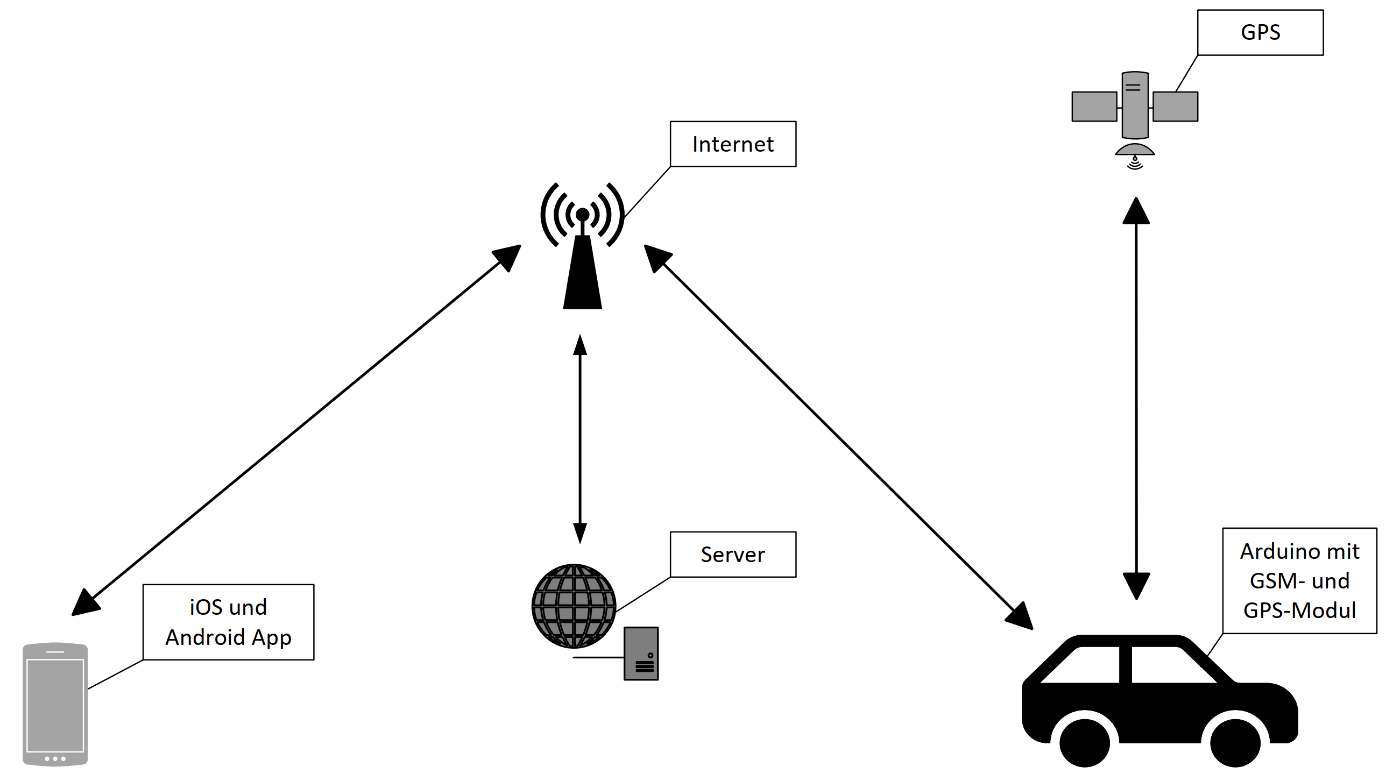
\includegraphics[width=1\textwidth]{Bilder/Konzept_Konzept.png}
		\caption{Systemkonzept}
		\label{konzept}
	\end{center}
\end{figure}
Im Fahrzeug wollen wir einen Arduino Uno zusammen mit einem passenden GSM- und GPS-Modul platzieren. Dieser ermittelt in bestimmten Zeitintervallen die aktuelle Position des Fahrzeugs und schickt die Koordinaten über die GSM-Verbindung an unseren Webserver. Dieser verarbeitet diese Daten und stellt sie anschließend so bereit, dass die Apps beider Betriebssysteme die aktuellen Koordinaten abfragen können.
	
	\chapter{Entwicklung}
	\section{Arduino}
\subsection{Ausstattung}
Um den Zielen, die wir uns für unseren Prototypen gesetzt haben, gerecht zu werden, ist der Arduino mit einem Sim 808 Module sowie entsprechenden GPS und GSM Antennen ausgerüstet.
\\
\\
Verbunden sind das Modul und die Antennen mit Hilfe eines Shields. Es handelt sich um ein Shield des Models OAS808SIM und ist von der Firma MakerFabs.
\\
\\
Die Stromversorgung erfolgt mittels vier BRC 18650 4200mAh Batterien, die in Reihe geschaltet sind. 
\subsection{Software}
Die Kontrolle des Shields erfolgt mittels UART und entsprechenden AT-Befehlen. Die erforderlichen Befehle sind zusammen mit einer kurzen Erklärung nachfolgend  in den Abbildungen \ref{Gsm_http} und \ref{GPS} aufgelistet.

\begin{figure} [H]
 \begin{center}
		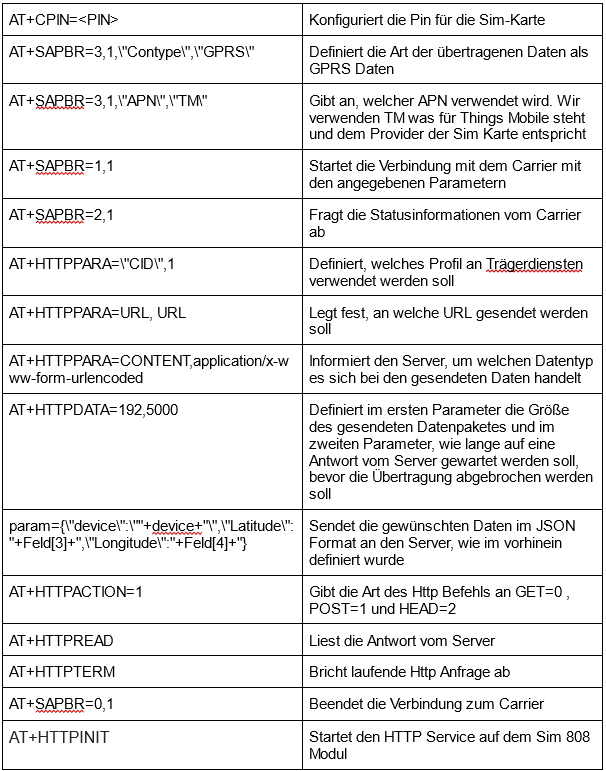
\includegraphics[width=1\textwidth]{Bilder/Arduino_Befehlstabelle_1.png}
		\caption{GSM und Http-Befehle}
		\label{Gsm_http}
	\end{center}
\end{figure}
\begin{figure} [H]
 \begin{center}
		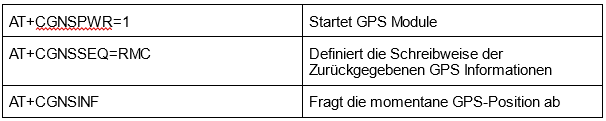
\includegraphics[width=1\textwidth]{Bilder/Arduino_Befehlstabelle_2.png}
		\caption{GPS-Befehle}
		\label{GPS}
	\end{center}
\end{figure}
\subsection{Aufbau Code}
Der Code ist wie ein Standard-Mikrocontroller-Code aufgebaut und besitzt zwei Unterfunktionen, die hier kurz grafisch in Abbildung \ref{PAP} dargestellt werden.
\begin{figure} [H]
	\begin{center}
		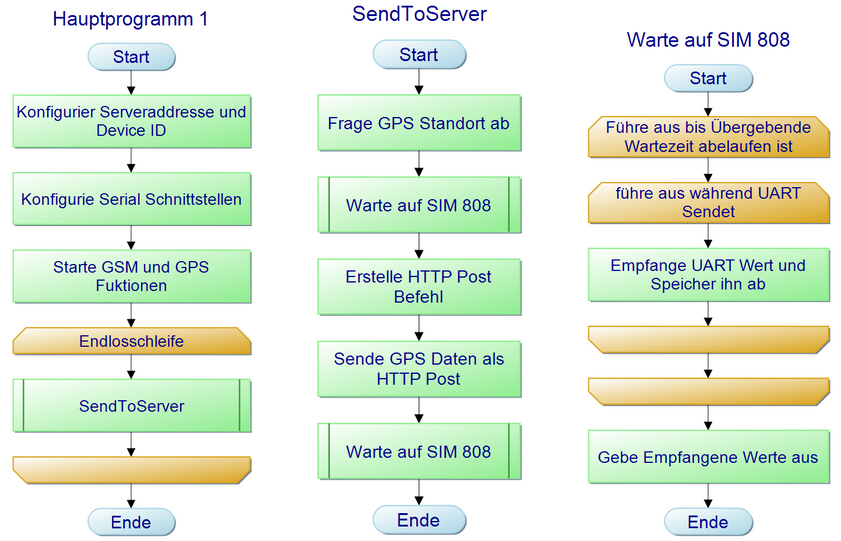
\includegraphics[width=1\textwidth]{Bilder/Arduino_Codeaufbau.png}
		\caption{Programmablaufplan}
		\label{PAP}
	\end{center}
\end{figure}
Der Arduino macht in der momentanen Prototyp Version nichts anderes, als das Sim 808 Modul zu steuern. Dafür gibt es drei Funktionen:
\\
\\
Eine Funktion, welche die Kommunikation mit dem Sim Modul erleichtert, eine weitere Funktion für die Abfrage des momentanen Standortes und eine dritte, um die Kommunikation mit dem Server zu erlauben. 
\\
\\
Mit der Funktion wart() wird zum einen das Pausieren für die Bearbeitungszeiträume geliefert und zum anderen die Ausgabe des Sim Moduls an den PC zum Debuggen geschickt. 
Die Funktion gpsDaten fragt den aktuellen Standort ab und die Funktion SendToServer sendet die zu übermittelnden GPS Daten an den Server.
Der Code ist in C geschrieben, da diese Programmiersprache für unsere Zwecke ausreichend performant ist.

\subsection{Entwicklungsprozess}
Der Entwicklungsprozess ist in mehreren Stufen erfolgt. Zunächst wurde mittels eines einfachen Programms die Funktionalität der GPS-Antenne überprüft, da wir dafür noch keine Sim-Karte benötigten. Zur Implementierung der Standortabfrage soll zum ersten Mal die UART-Schnittstelle zum Board konfiguriert werden. Nachdem die UART-Schnittstelle konfiguriert wurde, haben wir die Funktion wart() entwickelt, um die Kommunikation mit der UART-Schnittstelle zu erleichtern. Mit Hilfe der wart() Funktion konnten wir nun auf die Antwort von der UART-Schnittstelle warten und dies auf dem Computer zum Debuggen ausgeben. Das Senden und Empfangen von Informationen über UART funktionierte also und anschließend haben wir die Abfrage der GPS-Daten realisiert. Nachdem wir die entsprechenden Befehle gefunden hatten, war dies einfach zu realisieren.
\\
\\
Da die ersten Tests jedoch auf dem Dachboden ausgeführt wurden und das Dach aus Metall ist, konnte zunächst kein Signal empfangen werden. Nachdem wir das Problem erkannt hatten, haben wir alle zukünftigen Test an einer besser geeigneten Position durchgeführt.
\\
\\
Die Standortabfrage funktionierte nun, sodass wir im nächsten Schritt zum Testen des GSM-Moduls und der Sim-Karte das Senden von SMS realisiert hatten. An dieser Stelle haben wir lediglich die bereits erstellten Funktionen genutzt und die Befehle für die SMS-Kommunikation hinzugefügt. Dabei ist aufgefallen, dass beim erstmaligen Nutzen des GSM-Moduls nach dem Einschalten immer der PIN zum Entsperren erforderlich ist. 
\\
\\
Nachdem wir die Kommunikation mit dem GSM Modul ermöglicht hatten, haben wir die Kommunikation mit dem Server realisiert.
Nachdem wir hierfür die richtigen Befehle gefunden hatten, haben wir zunächst Testdaten per HTTP POST an einen Test-Server gesendet, der einfach nur seine empfangen HTTP POSTs anzeigt. Danach haben wir das Senden von Daten im JSON-Format an unseren Server realisiert. Aus Netzwerksicht mussten wir nur die Serveradresse ändern.  Damit der Server die empfangenden Daten nutzen kann, mussten wir dann jedoch noch den Daten-Sendebefehl neu konfigurieren. Da wir über die UART-Schnittstelle nur Strings schicken können, mussten wir die Formatierung für die zu sendenden Daten anders einstellen und diese  dann beim versendeten String berücksichtigen. 
\\
\\
Nachdem die Kommunikation mit dem Server erfolgreich funktioniert hatte, haben wir die einzelnen Teile zusammengefügt. Hierfür mussten wir den GPS-Antwort-String verarbeiten. Um die benötigten Werte zu erhalten, haben wir den String immer an den Kommata in kleinere Strings unterteilt und über die vordefinierte Struktur des Strings ermittelt, welche Werte der Längengrad und der Breitengrad sind. Dies Werte haben wir für zukünftige Erweiterungen beziehungsweise Funktionalitäten zwischengespeichert und binden diese in den zu sendenden String ein.
\\
\\
Wir haben dabei den Datentyp String der erhaltenen Daten bewusst nicht geändert, da dies sonst dazu führt, dass Nachkommastellen weggelassen werden, was die Standortbestimmung verzerrt.
\subsection{Aufbau Hardware}
Für die Stromversorgung müssen die Akkus an den Vin (\textit{Eingangsspannung}) Pin und den GND (\textit{Masse}) Pin angeschlossen werden. Da das Shield diese Pins einfach durch schaltet, können wir die Konstruktion trotz Shield so verwenden.
\begin{figure} [H]
	\begin{center}
		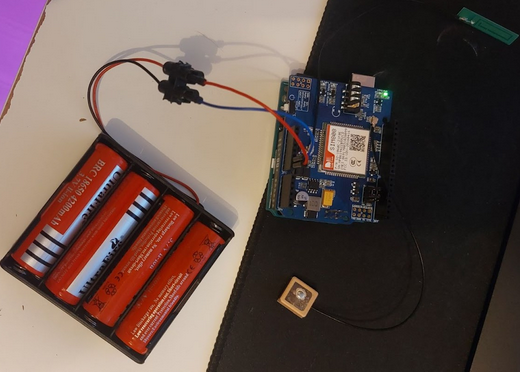
\includegraphics[width=1\textwidth]{Bilder/Arduino_Aufbau.png}
		\caption{Systemaufbau für das KFZ}
		\label{hw-system}
	\end{center}
\end{figure}
Der Vorteil dieser Konstruktion ist, dass sie sehr kompakt ist und somit leichter im Auto versteckt werden kann. Ein weiterer Vorteil dieser Bauweise ist, dass für den Fall, dass später durch Erweiterungen die Akkulaufzeit nicht ausreicht, einfach weitere Akkus parallel hinzugefügt werden können.

\subsection{Probleme}
Die Probleme, die bei der Entwicklung des Controllers aufgetreten sind, lassen sich in zwei Kategorien unterteilen. Zum einen gab es technische Probleme und zum anderen logistische Schwierigkeiten.
Das Problem bei der Beschaffung der GSM-Module war, dass diese meist aus China importiert werden mussten, was dazu geführt hat, dass wir unter langen Wartezeiten gelitten haben. Von den vier bestellten Modulen wurden zwei nicht geliefert (\textit{die Bestellung wurde vom Lieferanten gecancelt}). Des Weiteren konnte eines der Module nur über eine bereitgestellte Software verwendet werden.
\\
\\
Die technischen Probleme sind zum Teil auf die schlechte Dokumentation des Arduino Shields zurückzuführen. Zum einen fehlt die Information für die richtige Baudrate für die UART Schnittstelle, welche über strukturiertes Testen herausgefunden werden musste. Das Problem hierbei war, dass das Modul entsprechend keine Fehlermeldung zurückgeben konnte, da die Kommunikation zwischen Modul und Arduino selbst gestört war und  nichts zurückgeben wurde:
\begin{figure} [H]
	\begin{center}
		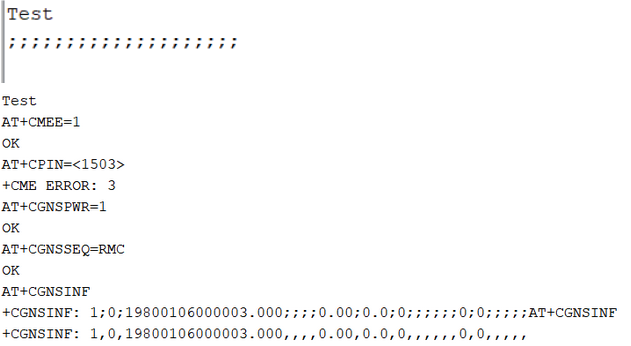
\includegraphics[width=1\textwidth]{Bilder/Arduino_Probleme.png}
		\caption{fehlerhafte und korrekte Ausgabe}
		\label{Arduinoproblem}
	\end{center}
\end{figure}
In Abbildung \ref{Arduinoproblem} sieht man zunächst, wie die fehlerhafte Ausgabe aussieht. Unter dieser ist zm Vergleich die richtige Ausgabe abgebildet.
\\
\\
Auch die AT-Befehle, welche zur Kommunikation mittels HTTP dienen sollten, haben nicht entsprechend funktioniert. Gelöst werden konnte das Problem, indem die Befehlskette verwendet wird, mit der jedes Datenpaket einzeln und manuell konfiguriert werden kann. Entsprechend mussten die Pakete als IOT-HTTP-Paket definiert werden und die Netzbetreiber-Daten sowie Paketinformationen für die Verbindung eingestellt werden.
\\
\\
Des weiteren hat das GSM-Modul die Kommunikation mit einer normalen Vodafone Sim-Karte nicht aufbauen können. Die Verzögerung, eine geeignete Prepaid Karte zu bekommen, hat den Zeitrahmen für diesen Teil erheblich nach hinten verschoben.
Das Problem an diesem Fehlern war, dass das Modul nur ERROR 3 zurückgegeben hat, was als \textit{“Operation nicht erlaubt”} definiert ist. Es wird dabei aber nicht genauer spezifiziert, warum diese Operation nicht erlaubt ist. Dies hat das Troubleshooting weiter erschwert.
\\
\\
Für die GPS-Abfrage haben sich zwei wesentliche Probleme ergeben. Das am schwierigsten zu lösende Problem war, dass die benötigten Befehle nicht in der richtigen Dokumentation zu finden sind, sondern nur in einigen Beispiel-Programmen vom Shield Hersteller. Das andere Problem ist, dass das GPS-Signal beim ersten Konfigurieren (\textit{Einstellen der internen Uhr}) guten Empfang braucht.


	\section{Webserver}
\subsection{Einleitung / Notwendigkeit}
Damit die vom Arduino ermittelten Standortdaten des Fahrzeugs an die Apps weitergeleitet werden können, benötigt es eine Zwischeninstanz. Diese soll die empfangenen Daten aufbereiten und sie anschließend so bereitstellen, dass sie einfach von den Apps abgefragt werden können.
In einem zweiten Entwicklungsschritt soll dann der Sicherheitsaspekt der Daten berücksichtigt werden. Hierfür sollen Verschlüsselungsalgorithmen implementiert werden, sodass die Daten nur von den Apps entschlüsselt und ausgewertet werden können.

\subsection{Einrichtung des Webservers auf einem Raspberry Pi}
Der HTTP-Webserver soll auf einem Raspberry Pi mit Hilfe des „lighttpd“-Webservers erstellt werden. Die Installation und Einrichtung desselbigen gestaltete sich relativ einfach. Zunächst musste das entsprechende „lighttpd“-Paket auf dem Raspberry Pi installiert werden. Im nächsten Schritt mussten noch ein paar Berechtigungen erteilt werden. Nach einem Neustart von lighttpd war die Einrichtung soweit fertig und der Webserver war aktiv. Alle Dateien und Skripte, die der Webserver bereitstellt und bearbeitet liegen im Verzeichnis „/var/www/html“.
Damit der Server später auch von außerhalb erreichbar ist, waren noch einige Arbeitsschritte zu erledigen. Zuerst musste der Raspberry Pi eine statische IPv4-Adresse erhalten, wir setzten diese auf 192.168.178.215. Die .215 wurde deshalb ausgewählt, weil der Bereich der automatischen Adresszuweisung von den meisten DHCP-Servern nur von .0 bis .200 geht und somit eine doppelte Vergabe sehr unwahrscheinlich ist.
Bei DYNDNS handelt es sich um einen Service, der es ermöglicht, Domains mit dynamisch wechselnden IP-Adressen im Internet zu verwalten. Dieser Service ist notwendig, da der heimische Router vom Provider in regelmäßigen Abständen eine neue, externe IP-Adresse zugeordnet bekommt und somit der Raspberry Pi bzw. der darauf aktive Webserver nach einem "IP-Wechsel" nicht mehr über das Internet erreichbar wäre. Bei Nutzung eines DYNDNS Anbieters, bleibt der Raspberry Pi bzw. der Webserver weiterhin unter seinem vergebenen Hostnamen erreichbar. Damit ein solcher Service genutzt werden kann, ist es notwendig, sich bei einem DYNDNS-Anbieter einen Account anzulegen. Für diese Arbeit wurde sich aufgrund einer persönlichen Empfehlung für Securepoint DYNDNS entschieden. Auf deren Webseite konnte nach der Erstellung eines Benutzerkontos ein IPv4-Host hinzugefügt werden. Dafür wurde neben der IP-Adresse des Raspberry Pi der Hostname eingetragen, welcher dann automatisch eine Domainerweiterung des DYNDNS Anbieters erhalten hat.
Im letzten Schritt musste nun der heimische Router so konfiguriert werden, dass ein Zugriff auf den Webserver von außerhalb des Heimnetzwerks erlaubt ist. In unserem Fall handelt es sich beim Router um eine FRITZ!Box, bei welcher diese Einstellungen einfach vorgenommen werden konnten.  Dafür musste zunächst eine neue Freigabe für das Gerät „Raspberry Pi“ hinzugefügt werden. Anschließend wird als Anwendung „HTTP-Server“ und damit Port 80 ausgewählt. Zusätzlich musste dann noch das DYNDNS in der FRITZ!Box konfiguriert werden. Dafür wird eine Update-URL des DYNDNS-Anbieters sowie der Domainname und die Benutzerinformationen benötigt. Damit waren alle notwendigen Einstellungen vorgenommen und er Webserver ist nun von überall erreichbar.
Zusätzlich haben wir die Software „VNC Server“ auf dem Raspberry Pi installiert. Mit Hilfe dieser Software und dem entsprechenden Client „VNC Viewer“ auf einem PC oder Laptop kann eine Remotedesktopverbindung zum Raspberry Pi hergestellt werden. Dies ist besonders auch in Zeiten von Lockdowns und Online-Vorlesungen sowie digitalen Gruppenmeetings eine wichtige Funktion, da so von überall an dem Raspberry Pi gearbeitet werden kann.

\subsection{Probleme mit dem Raspberry Pi}
Während der ersten Wochen der Projektarbeit mussten wir leider alle paar Tage feststellen, dass keine Verbindung per VNC zum Raspberry Pi hergestellt werden konnte. Wir vermuteten zunächst keinen dramatischen Fehler, denn nach einem Neustart funktionierte wieder alles. Dieser Fehler trat allerdings doch mit einer gewissen Regelmäßigkeit auf und nachdem ein erstes PHP-Skript auf unserem Webserver lief, konnten wir feststellen, dass dieses auch regelmäßig nicht erreichbar war. Der Fehler lag also eindeutig nicht nur an der VNC-Software, sondern es scheint generelle Verbindungsprobleme des Raspberry Pi zu geben.
Deshalb versuchten wir doch genauer herauszufinden, wo der Ursprung des Verbindungsverlustes ist. Nach einigem Recherchieren und dem Sichten diverser Log-Files auf dem Raspberry Pi konnten wir die Fehlermeldung „brcmf\_cfg80211\_scan: scan error (-110)“ für die Verbindungsabbrüche ausfindig machen. Bei diesem Fehler handelt es sich um ein Verbindungsproblem des WiFis des Raspberry Pi’s. Dieser Fehler ist nicht unbekannt und mögliche Lösungen werden in diversen Internetforen diskutiert. Allerdings scheint keine der vorgeschlagenen Workarounds generell zu funktionieren, außer ein wie auch von uns praktiziertes, regelmäßiges Neustarten. Bevor wir diese alle ausprobieren und im ungünstigsten Fall eine Menge Zeit ohne Ergebnis verschwenden würden, entschlossen wir uns einfach dazu, den Raspberry Pi per LAN-Kabel direkt mit der Fritzbox zu verbinden. Nachdem dann auch nach über zwei Wochen keine Verbindungsabbrüche registriert wurden, konnten wir dieses Problem als gelöst ansehen und uns wieder anderen Aufgaben des Projekts widmen.

Im Verlauf der weiteren Programmierung der PHP-Skripte stellte sich heraus, dass die PHP-Version 7.3 auf dem Raspberry Pi veraltet war und einige nützliche Funktionen nicht unterstützt. Deshalb wurde die Version 7.3 deinstalliert und anschließend mit PHP 8.0 eine der aktuellen Versionen installiert. Allerdings lief entweder die Deinstallation der alten oder die Installation der neuen Version nicht fehlerfrei. Nach einigem Suchen in verschiedenen Log-Files stellte sich heraus, dass fälschlicherweise die Socket-Datei „php7.3-fpm.sock“ der Version 7.3 vom lighttpd-Server versucht wurde zu öffnen. Diese existierte aber natürlich nach der Deinstallation nicht mehr. Mit PHP 8.0 wurde eine entsprechende, neue Datei „php8.0-fpm.sock“ im gleichen Dateipfad „/var/run/php“ bereits erzeugt. In der Konfigurations-Datei „15-fastcgi-php.conf“ im Verzeichnis „/etc/lighttpd/conf-enabled“ ist der Pfad der vom lighttpd-Server zu nutzenden Socket-Datei hinterlegt. Allerdings ist es nicht möglich, diese Datei einfach mit Hilfe eines Texteditors auf dem Raspberry Pi zu verändern. Dafür benötigt es höhere Benutzerrechte. Die Datei lässt sich auch über die Kommandozeile öffnen und bearbeiten. Dabei ist es wichtig den Zusatz „sudo“ vor jeden Befehl zu schreiben, da somit für den folgenden Befehl die notwendigen höheren Rechte temporär gewährt werden. So war es möglich, in der Datei „15-fastcgi-php.conf“ den Pfad der Socket-Datei auf die aktuelle Datei von PHP-Version 8.0 zu ändern. Im Anschluss musste der lighttpd-Server noch einmal neu gestartet werden, sodass alle Änderungen übernommen werden konnten.

\subsection{Grundsätzliche Überlegungen}
Bevor es ans konkrete Programmieren verschiedener HTML- oder PHP-Skripte geht, wollte wir uns zunächst überlegen, was denn grundsätzlich auf dem Server passieren soll. Auf jeden Fall benötigen wir ein Skript, das Daten nutzen und weiterverarbeiten kann, die an seine URL (Uniform Resource Locator) übermittelt wurden. Darüber hinaus ist es sicherlich sinnvoll und möglicherweise sogar notwendig, das Bereitstellen von Daten für die Apps in einem separaten Skript zu realisieren. Zusätzliche Skripte für zum Beispiel eine Verschlüsselung der Daten sind gegebenenfalls zu einem späteren Zeitpunkt noch interessant.
Auch wenn der GPS-Sensor am Arduino neben den Längen- und Breitengraden noch viele andere Informationen erfasst, reicht es für unser primäres Projektziel aus, nur die Koordinaten an den Webserver zu senden. Um die Koordinaten-Paare bei der Weiterverarbeitung in den Apps unterscheiden zu können, soll der Webserver die Daten noch mit dem aktuellen Zeitstempel verknüpfen.
Sowohl die Daten, die der Arduino an den Webserver übermittelt als auch die Daten, die der Webserver für die Apps wieder bereitstellt, sollen im JSON-Format (JSON = JavaScript Object Notation) übertragen werden. Dieses Format ist einerseits leicht lesbar und andererseits ist es unabhängig von Programmiersprachen und somit universell nutzbar.

Über mögliche Sicherheitsaspekte unserer Datenübertragung dachten wir anfangs nicht wirklich nach, da eine an sich funktionierende Kommunikation zwischen den verschiedenen Teilnehmern erstmal im Vordergrund stand. Lediglich die Überlegung, wie man verhindern kann, dass nicht jeder beliebige Internetnutzer irgendwelche Daten an unseren Webserver schickt, beschäftigte uns am Anfang des Projekts. Es lässt sich natürlich nicht verhindern, dass andere Geräte versehentlich oder auch absichtlich irgendwelche Daten an unseren Webserver bzw. an ein dort laufendes PHP-Skript senden. Aber wir können dieses Skript so programmieren, dass nur bestimmte empfangene Daten auch weiterverarbeitet werden. Um dies zu realisieren, muss jedes Gerät eine von uns manuell vergebenen Geräte-Identifikationscode (Geräte-ID) zusammen mit den Nutzdaten verschicken. Diese Geräte-IDs sind 20-stellige, alphanumerische Werte, die wir einmal zufällig generiert haben und die in der txt-Datei „allowed\_devices.txt“ lokal auf dem Raspberry Pi gespeichert sind. So kann später darauf zugegriffen werden und ein Abgleich erfolgen, ob die mitgesendete Geräte-ID bei uns bekannt ist. Wenn dies nicht der Fall ist, sollen diese Daten nicht weiterbearbeitet werden.
Es ist klar, dass auch diese Sicherheitsvorkehrung nicht besonders stark ist, solange die Geräte-IDs unverschlüsselt und quasi frei zugänglich auf dem Server gespeichert sind. Aber es ist ein erstes Mittel, um zumindest einfache Störversuche zu unterbinden und auch uns selbst vor möglichen Übertragungsfehlern zu schützen.

Es ist sehr wahrscheinlich, dass nicht alle Projektteile mit der gleichen Geschwindigkeit bearbeitet werden und somit einzelne Teile unterschiedlich schnell in einem testfähigen Stadium sind. In diesem Fall betrifft das die GSM-Sendeeinheit des Arduinos und die einzelnen Skripte des Webservers. Damit grundsätzliche Funktionalitäten der Skripte möglichst schon während der Entwicklung getestet werden können, ohne dass erst auf den Projektteil des Arduinos gewartet werden muss, wollten wir eine einfache Anwendung für einen Windows-PC entwickeln. Die Entscheidung fiel hier relativ schnell auf die Programmiersprache Python, da wir diese auch schon zuvor in einigen Studienprojekten benutzt hatten und sie für den hier gedachten Einsatzzweck eine einfache und schnelle Umsetzung verspricht.

\subsection{Testporgramme}
Im Verlauf der Programmierung der PHP-Skripte auf dem Webserver wurden insgesamt drei Python-Skripte geschrieben, um die Funktionen auf dem Webserver zu testen.
Das erste Python-Skript heißt „Senden.py“. Mit ihm soll getestet werden, ob gesendete Daten beim Webserver ankommen und auch weiterverarbeitet werden können. Dafür werden neben einer gültigen Geräte-ID auch je eine Variable für den Breitengrad (Latitude) und den Längengrad (Longitude) mit frei gewählten Startwerten deklariert. Ebenso wird die URL des empfangenden Skripts auf dem Webserver („http://retrorbit.spdns.de/get\_Data.php“) als Variable gespeichert. Der restliche Code ist eine endlose while-Schleife, in der die aktuellen Daten ins JSON-Format gebracht und dann mittels HTTP-POST an die gespeicherte URL gesendet werden. Danach folgt noch eine kurze Wartezeit von 5 Sekunden sowie eine Inkrementierung der Latitude und eine Dekrementierung der Longitude jeweils um den Wert 1.
Im zweiten Python-Programm mit dem Namen „Abfragen.py“ werden innerhalb einer endlosen while-Schleife die aktuellen Werte vom Webserver bzw. von der Webseite „http://retrorbit.spdns.de/provide\_Data.php“ per HTTP-GET abgefragt und die Daten im JSON-Format ausgegeben.
Das dritte Python-Skript heißt „Störer.py“ und gleicht dem „Senden.py“-Skript. Mit diesem sollten zeitgleich entweder beliebige oder auch vom Format her gleiche Werte an das „get\_Data.php“-Skript gesendet werden. So wollten wir überprüfen, ob die Sicherheitseinrichtung mit den Geräte-IDs tatsächlich funktioniert.

\subsection{Erstellen der PHP-Skripte zum Empfangen und Bereitstellen von Daten}
\textbf{Erläuerungen zum Code }Bei allen drei übermittelten Parametern, also Geräte-ID, Latitude und Longitude, wird immer eine Prüfung durchgeführt, bevor deren Werte tatsächlich in Variablen des PHP-Skripts geschrieben werden. Die Struktur dieser Prüfung ist bei allen drei Parametern identisch, bis auf den entsprechenden Bezeichner und den Variablennamen.
Die Variable übernimmt nur dann den Wert der \$POST Daten, wenn diese einerseits von „null“ verschieden sind und andererseits nicht leer sind. Dies wird realisiert, indem in einer if-Abfrage das Ergebnis der „isset“-Funktion mit der Bedingung, dass der \$POST Wert ungleich leer ist, über ein logisches UND verknüpft sind. Die „isset“-Funktion prüft dabei, ob die Variable existiert und sich von „null“ unterscheidet. Wenn diese Bedingungen allerdings nicht erfüllt sind, wird im else-Zweig mittels goto-Anweisung zum Ende des Skriptes gesprungen und eine Fehlermeldung ausgegeben. Die aktuell empfangenen Daten werden dann nicht weiterverarbeitet, sodass immer noch der vorherige Standort von der Seite „http://retrorbit.spdns.de/provide\_Data.php“ abgefragt werden kann.
Mit der Funktion str\_contains kann überprüft werden, ob ein String in einem anderen String enthalten ist. In unserem Fall wird so gecheckt, ob die Geräte-ID (\$device\_id) im String \$all\_devices enthalten ist, welcher alle Geräte-IDs aus der Datei „allowed\_devices.txt“ beinhaltet.
Die aus den \$POST Variablen übernommenen Werte für Latitude und Longitude werden dann zusammen mit den aktuellen Datumsinformationen in ein Array mit der Bezeichnung \$koor kopiert. Anschließend wird dieses Array noch in JSON codiert und als \$json\_koor gespeichert. Wichtig ist an dieser Stelle der zweite Parameter des json\_encode Befehls. Wenn hier nichts angegeben wird, werden alle enthaltenen Werte als String interpretiert. Für das Datum und die Uhrzeit ist das sinnvoll, für die Koordinaten hingegen eher nicht. Damit deren Werte auch als Zahlenwerte interpretiert werden, ist der Parameter „JSON\_NUMERIC\_CHECK“ zu setzen, welcher automatisch Zahlenformate erkennt und ins JSON Format übernimmt. Im letzten Schritt des „get\_Data.php“ Skripts wird der aktuelle Inhalt der Datei „Koordinaten.txt“ mit den Daten der JSON-codierten Variable \$json\_koor überschrieben.
Die Trennung für Datenempfang und Datenbereitstellung hat folgenden wichtigen, technischen Hintergrund. In dem Moment, in dem ein http-Request an das „get\_Data.php“ Skript gestellt wird – egal ob Daten mittels POST dorthin übermittelt werden oder nur die bereitgestellten Daten mittels GET abgefragt werden sollen – wird es einmal ausgeführt. Da bei einer reinen GET-Abfrage aber natürlich keine Daten mitgeschickt werden, wird der entsprechende PHP-Code zur Datenverarbeitung übersprungen und die Koordinaten mit „null“ gefüllt. Genau dies wird danach auch ausgegeben und von dem http-GET-Request ausgelesen. Somit ist es nicht möglich innerhalb eines PHP-Skripts Daten zu empfangen und bereitzustellen.
In der nachfolgenden Abbildung ist der grundsätzliche Programmablauf der beiden PHP-Skripte auf dem Webserver dargestellt, die die Datenverarbeitung sowie die Datenbereitstellung realisieren.
\begin{figure} [H]
	\begin{center}
		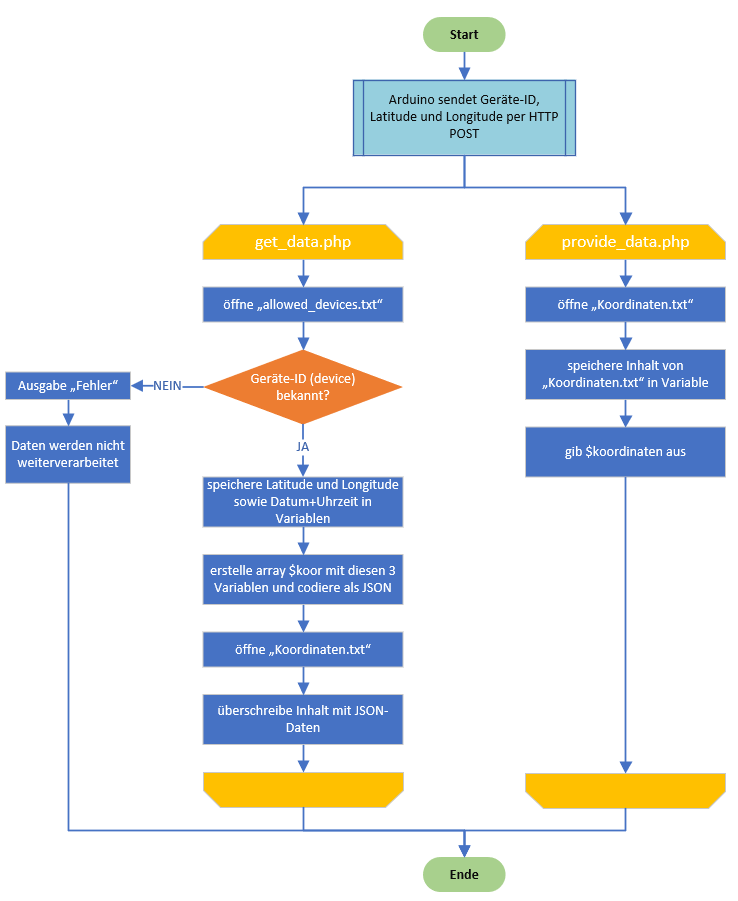
\includegraphics[width=1\textwidth]{Bilder/Webserver_PAP.png}
		\caption{Programmablaufplan Webserver}
		\label{server-pap}
	\end{center}
\end{figure}
\textbf{Probleme beim Senden vom Arduino }Nachdem das Skript „get\_Data.php“ in einem funktionsfähigen Zustand war und auch das Testen mit dem Python-Programm „Senden.py“ keine Fehler ergab, konnte zum nächsten Entwicklungsschritt übergegangen werden. Dieser besteht darin, die Kommunikation vom Arduino über das GSM-Modul zum Webserver herzustellen, sodass dort die gesendeten Daten auch weiterverarbeitet werden können.
Im Prinzip müssen im Programm auf dem Arduino nur die Koordinaten ins JSON Format gebracht werden und per http-POST an die URL „http://retrorbit.spdns.de/get\_Data.php“ gesendet werden. Es erforderte einige Versuche, bis das überhaupt funktionierte, allerdings konnten die Daten auf dem Webserver nicht richtig verarbeitet werden. Dies äußerte sich darin, dass in der Datei „Koordinaten.txt“ für Latitude und Longitude der Wert „null“ eingetragen war. Das Auslesen der Daten mittels POST auf der Seite des Webservers hat also nicht funktioniert. Die Ursache hierfür lag bei der Datenformatierung des Arduinos bzw. dem AT-Befehl zum Senden der Daten via GSM. Dabei werden die Daten immer als String versendet unabhängig von der ursprünglichen Form, welche dann als String angesehen wird. Deshalb funktionierten im PHP-Skript die \$\_POST Befehle für die einzelnen Parameter nicht mehr.
Mit diesem Wissen wurde das „get\_Data.php“ Skript nochmals angepasst und als „get\_Data2.php“ abgespeichert. Dieses ist im Prinzip genauso aufgebaut wie die ursprüngliche Version, jedoch wurden die einzelnen \$\_POST Befehle gegen einen normale Arraybezeichner (\$POST\_data) ausgetauscht. Dafür wird nach den Deklarationen der Dateinamen in Zeile 6 mit nur einem  \$\_POST der vom Arduino gesendete String ausgelesen und in der Variable \$Arduino\_Daten gespeichert. Es folgt eine JSON-Decodierung, sodass nun die einzelnen Parameter (Geräte-ID und die beiden Koordinaten) im Array \$POST\_data gespeichert und referenzierbar sind. Der Zugriff auf die einzelnen Werte geschieht jetzt also nicht mehr über die \$\_POST Befehle, sondern per Referenzierung auf das Array.

\subsection{Verschlüsselung der Daten}
\textbf{Hintergrund }Im aktuellen Zustand des Webservers und unserer Kommunikation allgemein werden die Koordinaten unverschlüsselt und damit für jedes Gerät bzw. jeden Nutzer klar lesbar auf der Seite „http://retrorbit.spdns.de/provide\_Data.php“ dargestellt. Sowohl aus datenschutztechnischer Sicht als auch im Interesse des späteren Kunden ist dies natürlich nicht. Deshalb ist es nötig, die bereitgestellten Daten zu verschlüsseln. Der wichtigste Punkt an dieser Stelle ist, dass die verwendeten Chiffrier- und Dechiffrieralgorithmen bzw. Bibliotheken sowohl von PHP als auch von den beiden Programmiersprachen der Apps unterstützt werden.
\\
\textbf{Symmetrische und asymmetrische Verschlüsselungsverfahren }Die Verschlüsselung unserer Nutzdaten, also Latitude, Longitude sowie die dazugehörigen Datumsinformationen, soll mittels eines symmetrischen Verschlüsselungsverfahren realisiert werden. Symmetrische Verschlüsselungs-verfahren sind einerseits sehr performant, selbst bei großen Datenmengen, und andererseits sind sie nur unter unverhältnismäßig großem Aufwand zu entziffern. Ein weit verbreiteter, frei verfügbarer Standard stellt dabei der „Advanced Encryption Standard“, kurz AES, den auch wir bei unserem Projekt nutzen wollen. Bei symmetrischen Verschlüsselungsverfahren wird für das Ver- und Entschlüsseln ein und derselbe Schlüssel benutzt. Beim AES kann dieser Schlüssel wahlweise 128, 192 oder 256 Bit lang sein, wobei gilt: Je länger der Schlüssel ist, desto höher ist auch die Sicherheit der verschlüsselten Daten. Bei der symmetrischen Verschlüsselung besteht aber ein wesentlicher Nachteil, denn der Schlüssel muss beiden Teilnehmern der Kommunikation bekannt sein. Wenn die Chiffrierung also auf Gerät A durchgeführt wird, muss neben den nun verschlüsselten Daten auch der AES-Schlüssel zu Gerät B übertragen werden. Je nach individuellen Gegebenheiten lässt sich dies ggf. auf einem zweiten Kommunikationsweg manuell durch den Menschen realisieren. In der Praxis ist das aber meist nicht möglich. Deshalb wird hier zusätzlich noch ein asymmetrisches Verschlüsselungsverfahren angewandt, mit welchem der AES-Schlüssel chiffriert wird. Diese Kombination beider Verschlüsselungsverfahren wird auch als Hybride Verschlüsselung bezeichnet.
Bei asymmetrischen Verschlüsselungsverfahren hat jeder Kommunikationspartner ein eigenes Schlüsselpaar bestehend aus einem öffentlichen und einem geheimen Schlüssel. Der öffentliche Schlüssel wird immer für die Verschlüsselung von Daten beim jeweilig anderen Teilnehmer genutzt und der geheime Schlüssel für die Entschlüsselung der empfangenen Daten auf dem eigenen Gerät. Der Vorteil ist hier, dass der öffentliche Schlüssel bei der Übermittlung an den Kommunikationspartner nicht extra geschützt werden muss. Eines der bekanntesten asymmetrischen Verschlüsselungsverfahren ist das nach seinen Entwicklern benannte RSA-Verfahren. Da dieses aber schon veraltet ist, werden wir mit der Elliptic Curve Cryptography ein zeitgemäßeres Verfahren nutzen.
\\
\textbf{Implementierung der Verschlüsselung auf dem Webserver }Der komplette Verschlüsselungsprozess ist in „encryption.php“ realisiert, also sowohl die Verschlüsselung der Nutzdaten als auch die Chiffrierung des AES-Schlüssels. Für die Übermittlung des öffentlichen Schlüssels wird zusätzlich das Skript „key\_from\_app.php“ erstellt. Allerdings ist die Implementierung noch nicht im Zusammenspiel mit einer der Apps getestet worden, da es hier Verzögerungen im Projekt gab, sodass das ganze Verschlüsselungsthema erst in naher Zukunft tatsächlich funktionsfähig sein wird. Für die symmetrische Verschlüsselung nutzen wir in PHP die Funktionen der „OpenSSL“ Bibliothek und für die asymmetrische Verschlüsselung kommen die Funktionen der „Sodium“ Bibliothek zum Einsatz, welche auch für die von uns verwendeten Programmiersprachen der Apps zur Verfügung stehen.
Als erstes werden die zu verschlüsselnden Nutzdaten (Koordinaten und Datum mit Uhrzeit) aus der Datei „Koordinaten.txt“ geladen. Anschließend wird das Verschlüsselungsverfahren auf AES-192-CTR festgelegt und ein entsprechend langer AES-Schlüssel generiert. CTR steht dabei für Counter Mode, welcher zusätzlich einen Initialisierungsvektor erfordert, welcher die gleiche Länge wie der AES-Schlüssel haben muss. Nachdem dieser Initialisierungsvektor generiert wurde, folgt die eigentliche Verschlüsselung unserer Nutzdaten mit der Funktion „openssl\_encrypt“. Weiter geht es mit der Generierung des Schlüsselpaares des Webservers für die asymmetrische Verschlüsselung mit der Funktion „sodium\_crypto\_box\_keypair()“.
Nun fehlt noch der öffentliche Schlüssel aus der App. Dieser wird aus der Datei „app\_key.txt“ geladen. Diese Datei wurde im Skript „key\_from\_app.php“ generiert und lokal auf dem Server gespeichert. Dieses Skript ist im Prinzip genau so aufgebaut wie das „get\_Data.php“ Skript, nur dass es entsprechend nur auf die beiden Parameter „Geräte-ID“ und „keypair2\_public“ abgestimmt ist. So findet auch hier zuerst eine Überprüfung statt, ob die gesendeten Daten von einem bekannten, erlaubten Gerät stammen.
Nachdem dann also alle notwendigen Schlüssel auf dem Webserver vorhanden sind, kann der AES-Schlüssel mit der Funktion „sodium\_crypto\_box()“, welche noch eine zusätzliche Zufallszahl (nonce) benötigt, verschlüsselt werden. Diese Zufallszahl wurde zuvor erzeugt und muss auch an den Empfänger für die Entschlüsselung übermittelt werden. Im nächsten Schritt werden wieder alle zu sendenden Variablen in ein Array (\$datenpaket) kopiert, siehe untenstehende Abbildung. Dabei ist es wichtig, dass alle Variablen bis auf die verschlüsselten Nutzdaten noch einmal mit base64 codiert werden, da sonst bei der JSON-Codierung des Arrays im nächsten Schritt nicht alle Zeichen der einzelnen Strings korrekt verarbeitet werden können. Bevor diese Strings dann allerdings in den Apps genutzt werden können, muss dort wieder eine base64 Decodierung erfolgen, um wieder das BYTES Format zu erhalten.
Im letzten Schritt werden nun die JSON codierte Variable \$json\_data in der Datei „Datenpaket.txt“ lokal abgespeichert. Diese Datei kann dann genau wie zuvor die Datei „Koordinaten.txt“ von dem Skript „provide\_Data.php“ geöffnet und deren Inhalt ausgegeben werden. So können die Entschlüsselungsparameter zusammen mit den verschlüsselten Daten von den Apps abgefragt werden.
\begin{figure} [H]
	\begin{center}
		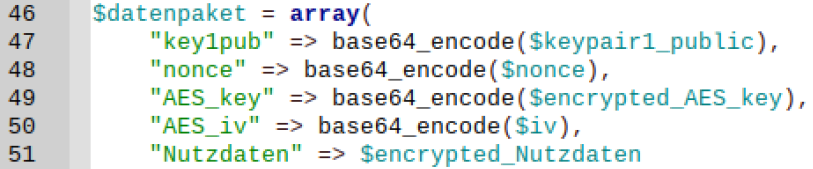
\includegraphics[width=1\textwidth]{Bilder/Webserver_verschluesslung.png}
		\caption{Datenpaket Webserver}
		\label{server-dp}
	\end{center}
\end{figure}
Der gesamte Ablauf der Skripte auf dem Webserver ist in der nachfolgenden Übersicht zur besseren Nachvollziehbarkeit noch einmal schematisch dargestellt.
\begin{figure} [H]
	\begin{center}
		\includegraphics[width=1\textwidth]{Bilder/Webserver_pap2.jpg}
		\caption{Skriptablauf Webserver}
		\label{server-script}
	\end{center}
\end{figure}

	
	\section{Android}

In diesem Kapitel wird das Konzept der mobilen Anwendung entwickelt. 
Das Kapitel enthält wesentliche Informationen und Schritte, die für die Entwicklung für eine Android-App erforderlich sind. 
Als Erstens wird das Konzept genau, was man in einer App-Entwicklung betrachten muss. Zweitens werden die Grundlagen vorgestellt.
Dann basierend auf dem Konzept des Projekts wird die Implementierung beschrieben.
\subsection{Mobile Apps}
Mobile Anwendungen werden unter Berücksichtigung von Faktoren wie Benutzerfreundlichkeit, Zugänglichkeit, Handbuch, Design, menschlicher Schnittstelle und Interaktion mit der Benutzererfahrung entwickelt. 
Es werden dabei unter anderem Features und Services genannt, die einen echten Mehrwert bieten und lassen die Anwendung attraktiv und innovativ erscheinen.
Über das volle Potenzial der App aufzudecken und konzeptionell zu benennen, ist wichtig, mögliche zukünftige App-Eigenschaften und -Funktionen über den Prototyp hinaus vorzuschlagen.\\
Was bei der Umsetzung der mobilen Applikation betrachten werden sollte:
\begin{itemize}
\item Die Brauchbarkeit und Nutzbarkeit 
\item Effizienz und Effektivität
\item Zuverlässigkeit
\item Saubere Interaktion
\item Dynamik und Flexibilität
\end{itemize}

\subsection{Entwicklungsumgebung: Android Studio}
Android ist das Betriebssystem und die Softwareplattform für mobile Geräte wie Smartphones
Telefone, Uhren, Fernseher oder Schnittstellen zur Kommunikation mit Fahrzeugen.
Android gehört Google und ist das am weitesten verbreitete Betriebssystem
Der weltweite Marktanteil von Smartphones liegt bei etwa 85 %.\\\\
Für die Entwicklung von Android Apps kann Android Studio verwendet werden. 
Es bezieht sich auf die offizielle integrierte Entwicklungsumgebung (IDE) für Android. Die IDE hilft beim Entwerfen und Entwickeln Android-Anwendungen mit vielen Hilfsfunktionen. Es hat gute integriertes Support-Capability-Management für Gradle, die Software für Android-Apps verwendete Build-System. Neue Abhängigkeiten sind normalerweise direkt unter verfügbar Quellcode-Editor, keine Notwendigkeit, Build-Skripte manuell zu bearbeiten. 
Android Studio hat auch viele andere sehr nützliche Funktionen, die oben nicht aufgeführt sind, wie z. B. eine integrierte Software-Versionskontrolle, effektive Debugging-Tools und einen sehr intelligenten Code-Inspektor\cite{AndSt}.
\subsection{Flutter}
Was ist Flutter? Flutter ist ein von Google entwickeltes Framework um nativ kompilierbare Anwendungen anhand einer einzigen Codebasis zu schreiben.
Flutter ist ein Open-Source-Framework von Google zur Entwicklung grafischer Anwendungen, die auf Mobilgeräten, Browsern und Computern ausgeführt werden. Der wichtige Aspekt sind die verschiedenen gemeinsamen Codebasen
Plattform und laufen mit nativer Geschwindigkeit. Die gleiche Anwendung kann also auch ohne viele Änderungen auf eine andere Plattform kompiliert werden. Flutter bietet umfangreiche Bibliotheken mit vorgefertigten UI-Elementen.Datenströme sind sehr einfach zu implementieren und stellen sicher, dass Benutzer immer auf dem neuesten Stand sind.\\
Die Verwendung des Flutter-Frameworks bietet mehrere Vorteile. Wie bereits erwähnt, liegt ein besonderer Fokus darauf, eine einzige Codebasis für viele Menschen zu verwenden Tree Form aufbauen. Das spart im Idealfall Zeit und Geld. Mit der “Hot Reload“ Funktion ermöglicht es Entwicklern, schnell und einfach Schnittstellen zu erstellen, neue Funktionen hinzuzufügen und  
Fehler schneller finden\cite{Flut}.
\subsection{Dart}
Flutter läuft auf Dart, der hauseigenen Programmiersprache von Google und basiert darauf.
Dart ist eine von Google entwickelte Computersprache. Sein ursprüngliches Ziel war es, JavaScript zu ersetzen und die neue Sprache zu werden
ein Netzwerk werden. Ihr derzeitiger Fokus liegt jedoch mehr auf JavaScript.
Der Code zum Konvertieren und über die Entwicklung von Multi-Plattform-Programmen.\\
Die Eigenschaften von Dart sind:
\begin{itemize}
\item Eine leichte zu lernende Sprache
\item Eine Gute Dokumentation
\item Eine hoher Leistungsfaktor
\item Eine klare und saubere Syntax
\item Hat unglaubliche Tools zur Unterstützung der App-Entwicklung
\end{itemize}
\subsection{Konzept: SchrödingerSAlarm}
Beim Projekt ist die Mobile Android app ein Wichtig Bauteil des Systems.
die Mobile App soll wie eine gewöhnliche Android App. Die App soll für jedes Android Smartphone kompatibel sein. Um mehr die Funktionalität der App wird durch die beiden Abbildungen dargestellt:\\
\textbf{Standard Fall:} Die App ist mit dem Webserver verbunden. Alle Informationen. die vom Webserver kommen, werden in der App angezeigt. Die Koordinaten sollen den Standort des Automobilfahrzeug auf einer Karte in der App angezeigt werden.
\begin{figure}[H]
            \centering
            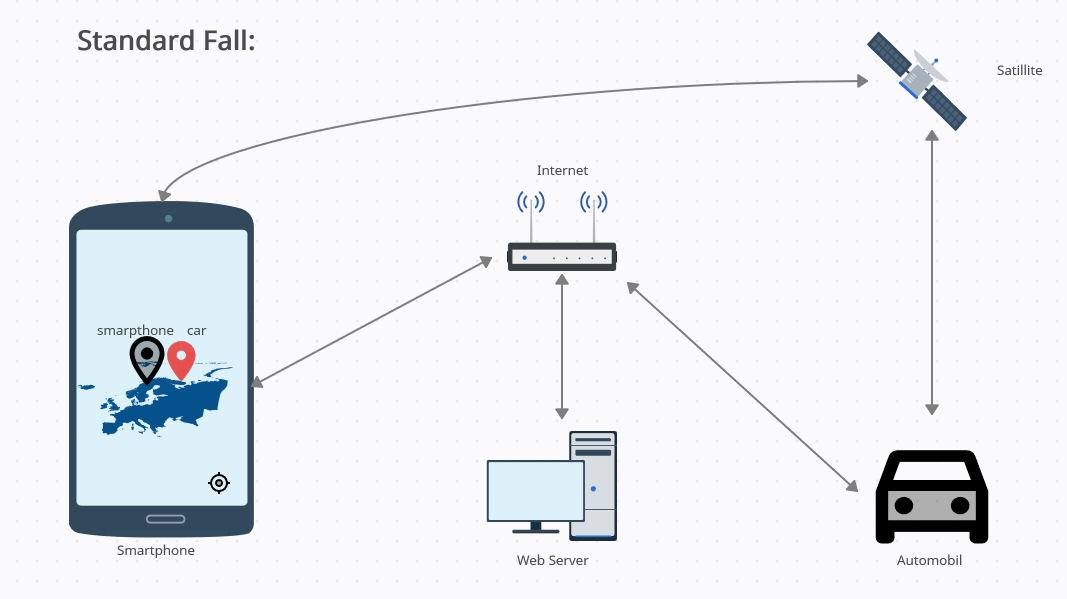
\includegraphics[width=1\textwidth]{Bilder/StandardFall.PNG}
            \caption{Konzept der Android App im AlarmFall}
\end{figure}
\textbf{Alarm Fall:} Im Falle das der Standort des Automobils sich bewegt und das Standort des Smartphones konstant ist, wird ein Alarm auf dem Handy ausgelöst und der Nutzer bekommt eine Push-Benachrichtigung.
     \begin{figure}[H]
            \centering
            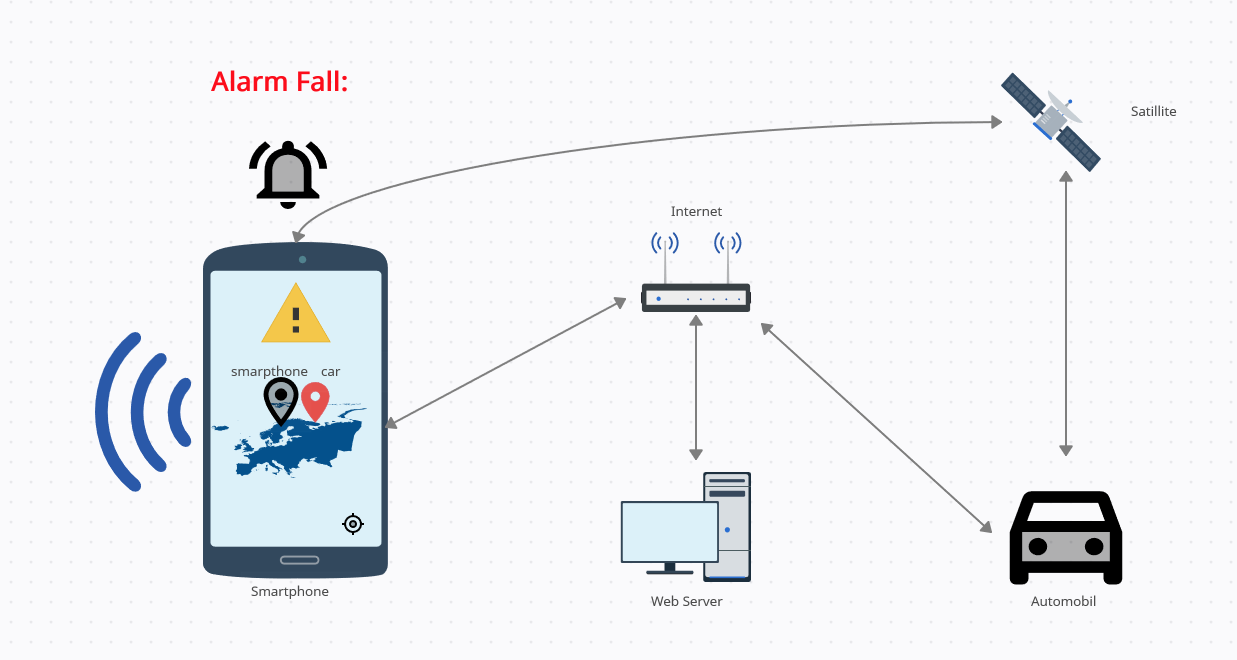
\includegraphics[width=1\textwidth]{Bilder/AlarmFall.PNG}
            \caption{Konzept der Android App im Standard Fall}
	
    \end{figure}
	
\subsection{Implementierung}
\subsubsection{Flutter Funktionalität}
Flutter ist sehr einfach zu verstehen und verkürzt die Lernkurve erheblich. Die Grundidee lautet: “Alles ist ein Widget“. Es ist dem Entwickler völlig selbst uberlassen wie er sein Projekt
strukturieren und hinsichtlich Architektur- und Entwurfsmuster logisch aufbauen möchte. Der Einstiegspunkt zu Flutter ist die main.dart-Datei oder die zentrale main()-Methode. Von dort aus ist es möglich, sich gegenseitig zu verschachteln und zu importieren. 
Die Entwicklung von Flutter beinhaltet hauptsächlich nur Widgets, weil alles hineingeschrieben wird.
Sogar ein einfacher Text “Teil“ wird als Widget festgelegt. 
\\
In Flutter gibt es wieder eine Baumstruktur “Widget Tree“. Jede betriebssystemspezifische Komponente, die man in Flutter verwenden möchte, muss zunächst von einem Flutter-Entwickler nativ entwickelt werden. Dies ist jedoch nur dann erforderlich, wenn die Anwendung auch der nativen Anwendung ähnlich sein soll. 
Aus den Basis-Komponenten aus den verschiedenen Paketen konnte man eigene Widgets schreiben. So kann sich ein eigener, abgerundeter Button beispielsweise durch eine Kombination aus RawMaterialButton, Text und Icon-Widgets darstellen lassen.
In Flattern werden Widgets jedoch als einfache Klassenvariablen über den Konstruktor der Klasse übergeben und können dort beliebig verwendet werden.
Durch die Klassenvariablen lassen sich Komponenten in
ihrem Aussehen sowie ihrer Funktionalität individualisieren und anpassen \cite{SDK}.\\
Es gibt zwei Arten von Komponenten in Flutter, die im Code explizit als solche benannt werden. Erstens ist es “Statful-Widgets“, die einen Zustand beibehalten oder verwalten können. Andererseits gibt es “Stateless Widgets“, die nur als statische, einfache Widgets dienen. Ein zustandsbehaftetes Widget erfordert immer eine zugeordnete createState()-Funktion. Eine Methode, die ein Zustandsobjekt (private Klasse) erstellt, das wiederum
verwaltet den Widget-Status. Abgesetzt durch Aufruf von setState ()
ruft die Methode build() auf, um die Komponente neu zu zeichnen. Die Methode build() wird beim Casting von Stateless verwendet
Ausgelagerte Widgets an das State-Widget in der privaten State-Klasse.\\
Das Styling in Flutter ist grundlegend speziell. Da alles ein Widget ist, so auch die Design Möglichkeiten realisiert.
Wenn man das Widget zentrieren möchten, könnte man beispielsweise das Center-Widget verwenden.
Um ein Widget von anderen Widgets entfernen möchte, muss dafür mit einem Padding-Widget umschlossen werden. Einfaches Beispiel in Text-Widget wird von einem zentralen Widget umgeben, das folgt
es ist wiederum vom Container-Widget umhüllt.\\\\
“Center“, “Raw“, “Column“, “Container“-Widgets und viele andere Widgets
sind die Bausteine in der Entwickelung von Flutter App.
\subsection{Implementierung SchrödingersAlarm App}
\subsubsection{Login Menü}
Das Starten der App ist hier Standard, wie eine jede App. Zuerst die Willkommensseite, in der soll ein Login Menü erscheinen. 
Jedes Gerät soll eine eigene IMEI und der PIN Code haben und den Kunden mitgeliefert. 
Diese beiden Informationen sind in der Datenbank auf der App eingefügt. Die Login-Seite beinhaltet zwei Komponenten.
Das Logo des Produkts wird oben direkt angezeigt. Unten sind zwei Eingabefeldern definiert,
in der man die Login-Informationen(IMEI/PIN) eingeben kann. Natürlich wird ein “Einloggen“ Button unter den Feldern gesetzt.
Der Login-Prozess hat ein genau definierten Mechanismus. In den beiden Feldern muss eine bestimmte Anzahl eingegeben werden. Ansonsten wird es nicht akzeptiert. Die IMEI muss 15 Ziffern beinhalten.  Die PIN code muss 6 Ziffern beinhalten.  Nur bei einer korrekten Dateneingabe wird man in der nächsten Seite geleitet.
Andernfalls erschient eine rote Fehlermeldung, die um korrekte Informationen bittet.\\\\
Die Umsetzung in Flutter ist simpel gestellt. Ein Widget wird als gesamte Seite implementiert. 
Wie vorher beschrieben ist, wird horizontale aufgeteilt. Der obere Teil ist das importierte Bild vom LOGO und der untere Teil von den Eingabefeldern. 
Diese Aufteilung wird mit einem “Column“ Widgets definiert. Der unter Teil wird auch in viele Widgets aufgeteilt. 
Darunter sind zwei Eingabefeldern und der “Einloggen“ Button.
 \begin{figure}[H]
            \centering
            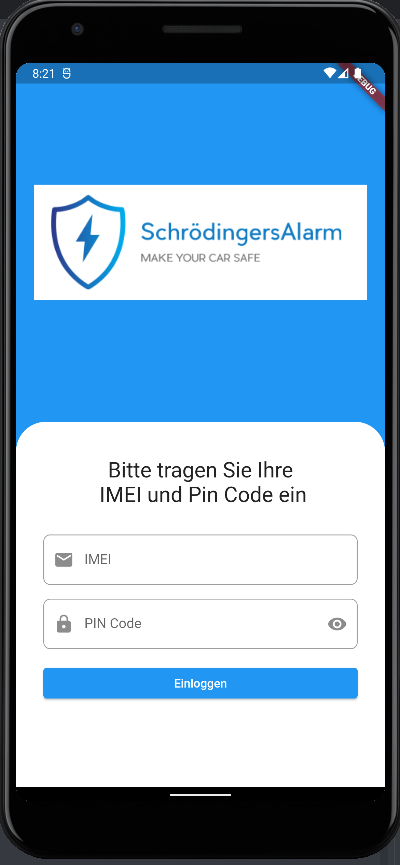
\includegraphics[width=0.5\textwidth]{Bilder/LoginIn.PNG}
            \caption{Android App: Login Seite}
    \end{figure}

\subsubsection{Hauptseite}
Nach erfolgreichem Login leitet die App den Nutzer auf der Hauptseite.
Auf der Hauptseite gibt es einer horizentalen Appbar von 3 Kategorien (Home/Status/Maps), links oben ein Menu item für Support und rechts oben ein logout item für das Ausloggen aus der App. 
Im Home wird das Logo und Standpunkt der aktuellen Lage angezeigt.
Wenn das Auto sicher gemeldet ist, wird ein grüner Kreis mit der Meldung “your car is safe“ angezeigt. 
Falls das Auto nicht im sicheren Zustand ist, wird ein roter Kreis mit der Meldung “Dangerous situation“.\\\\
Durch das Drücken auf „Status“ in der horizentalen Appbar, werden die Informationen, die aus dem Webserver kommen, in einem Text Widget angezeigt.
Wichtig hier ist auf eine Webserver Verbindung zu prüfen. Falls es eine Verbindung gibt, soll ein Grüne Verbindung Icon angezeigt werden.
Im Falle einer Störung wird ein Icon “nicht verbunden“ angezeigt.\\\\
Das dritte Item in der horizontalen Appbar ist die Karte. In der wird die Google Maps Anwendung in der App geöffnet.
Die Koordinaten, die von dem Webserver kommen, werden dann in einem Marker in der Google Maps Karte markiert. 
Dazu kommt der aktuelle Standort des Smartphones über den GPS in einem andren Marker angezeigt.\\\\
Falls die Koordinaten vom Webserver weit entfernt von den interpretierten Koordinaten vom GPS Smartphones ist, bekommt man eine Push-Benachrichtigung. Bei der Umrechnung werden Longtitude und Latitude von beiden Koordinaten abgezogen und den Beitrag von den beiden Werten gerechnet. 
Falls einer der beiden Werten höher als der festgelegten Wert ist, wird die App eine Push-Benachrichtigung erstellt.
 	\begin{figure}[H]
   \centering
            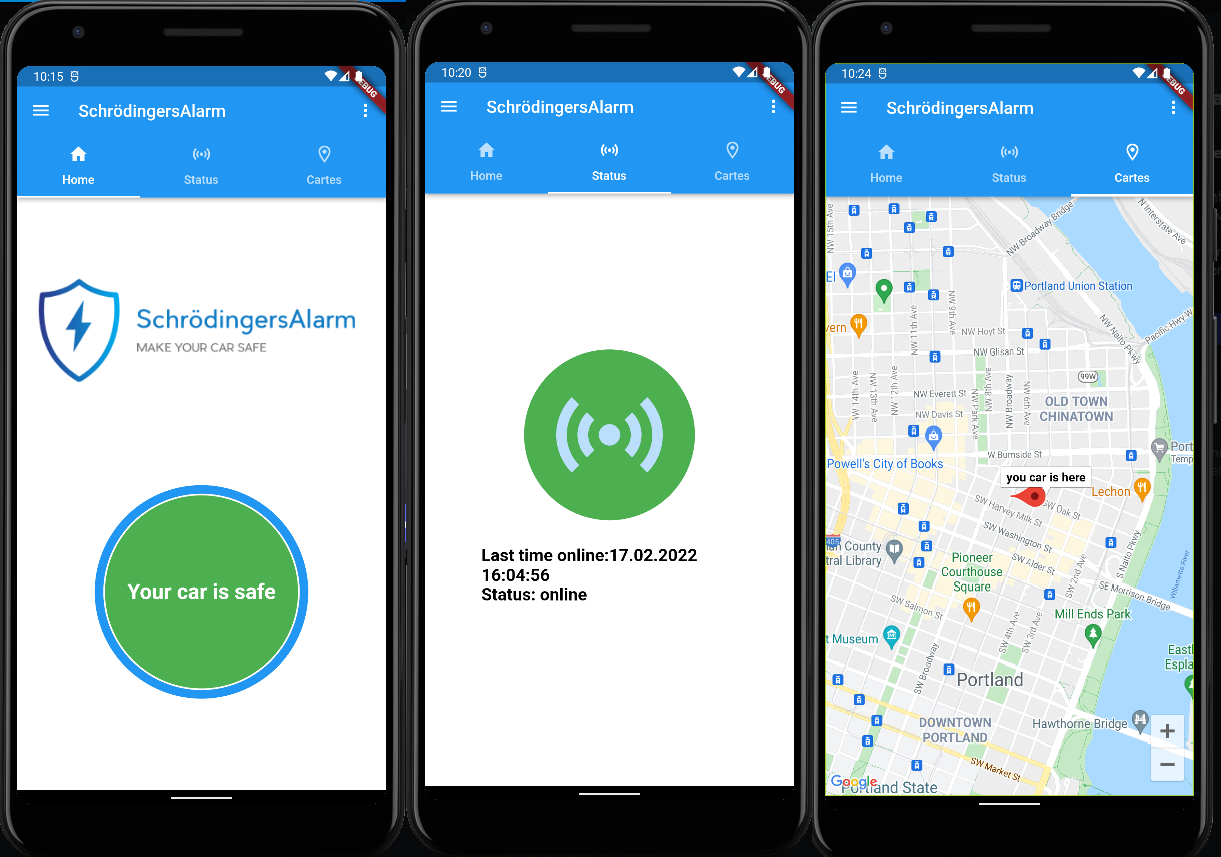
\includegraphics[width=0.75\textwidth]{Bilder/hauptseite.PNG}
		            \caption{Android App: Hauptseite}
    \end{figure}
		
	\section{App - iOS}
Um möglichst viele Endnutzer für unser Produkt zu erreichen, war es uns wichtig, für die zwei verbreitetsten Smartphone Betriebssysteme Apps bereitzustellen. Für die Entwicklung der iOS-App wurde die Sprache SwiftUI unter Nutzung der  kostenlosen IDE Xcode genutzt.  Da es sich hier um neues Terrain handelte, wurde mehr Zeit zur Einarbeitung und späteren Problemfindung benötigt, als anfänglich gedacht, weshalb diese App eher einem Design-Prototypen entspricht. 

\subsection{Xcode}
Mit Xcode können Programme für macOS, iPadOS, iOS, watchOS und tvOS entwickelt werden. Diese IDE ist für die Programmiersprachen Swift und Objective-C unter Verwendung der Cocoa-Frameworks vorgesehen, wobei aber auch die Programmiersprachen C und C++ verwendet werden können. Aufgrund seiner Modularität ist es jedoch auch möglich Programme in anderen Sprachen zu schreiben – beispielsweise in Java, Ruby, Perl oder Pascal. \cite{Ahmad2020}
\\
\\
Wie von Apple gewohnt, bietet Xcode eine übersichtliche wie aufgeräumte Benutzeroberfläche. Beim Starten eines neuen Projektes hilft ein Assistent bei den richtigen Einstellungen. Neben dem Programmieren von Apps unterstützt das Tool auch das visuelle Gestalten der späteren Benutzeroberfläche sowie das Testen und Debuggen von Software. \cite{Ahmad2020}
\\
\\
Die IDE kommt mit einem grafischen Interface-Design-Tool namens Interface Builder, über das Benutzeroberflächen entwickelt werden können. Menüs, Fenster, Controls und weitere visuelle Elemente lassen sich gestalten oder aus vorhandenen Objekten, aus einer integrierten Bibliothek ziehen. Alternativ können natürlich auch eigene entwickelt werden. Die Anbindung bestimmter Elemente an den dahinterliegenden Code (\textit{in Form von ausführbaren Aktionen beispielsweise}) ist mit dem Interface Builder ebenfalls möglich.\cite{Ahmad2020}
\\
\\
Für Xcode wurde sich einerseits entschieden, um später keine Komplikationen mit der Kompatibilität auf dem Endgerät zu riskieren. Bei der Recherche, welche IDE wir nutzen möchten, wurde relativ schnell klar, dass dies bei anderen kostenlosen IDE Tools passieren könnte. Andererseits überzeugten die vielen hinterlegten Simulatoren - von iPad, über Macbook bis hin zu sämtlichen iPhone Generationen ist alles dabei - welche ein Arbeiten mit schnellem Feedback auf unterschiedlichen Geräten ermöglichen, ohne diese physisch Zuhause haben zu müssen.

\subsection{SwiftUI}
Bei SwiftUI handelt es sich um ein GUI-Framework aus dem Hause Apple, welches auf MVVM\footnote{Model View ViewModel = ein Entwurfsmuster, zur Trennung von Darstellung und Logik der UI} basiert.
Es bietet Ansichten, Steuerelemente und Layoutstrukturen zum Deklarieren der Benutzeroberfläche einer App. Das Framework bietet Event-Handler für die Bereitstellung von Taps, Gesten und anderen Arten von Eingaben an der App sowie Tools zur Verwaltung des Datenflusses von den Modellen der App bis hin zu den Ansichten und Steuerelementen, die Benutzer sehen und mit denen sie interagieren.\cite{Inca}
\\
\\
Die App-Struktur wird mithilfe des App-Protokolls definiert und füllt sie mit Szenen, welche die Ansichten enthalten, aus denen die Benutzeroberfläche der entstehenden App besteht. Es können eigene benutzerdefinierte Ansichten erstellt werden, die dem Ansichtsprotokoll entsprechen, sowie  SwiftUI-Ansichten zum Anzeigen von Text, Bildern und benutzerdefinierten Formen mithilfe von Stapeln, Listen und mehr. \cite{Inca}

\subsection{Hauptkriterien an die Funktionalität}

Damit die App erkennt, ob sich das Auto bewegt oder nicht, muss sie mit dem Webserver kommunizieren können, um sich dort die vom Arduino gesendeten GPS-Daten zu holen. Zusätzlich muss eine Logik implementiert werden, welche bei eingeschaltetem System eine Veränderung der GPS-Daten erkennt und der Nutzer eine Benachrichtigung erhält. Weiterhin benötigen wir eine Funktion, dass die Koordinaten  nicht als plain-Text angezeigt werden, sondern direkt auf einer Karte, wie man es beispielsweise von Google Maps gewohnt ist. Eine weitere sinnvolle  aber eher optionale Implementierung wäre es, wenn die App erkennt, ob der Server gerade erreichbar ist und ein Icon dementsprechend die Farbe ändert.  Um die theoretischen Prozesse zu strukturieren und auch übersichtlich zu visualisieren, haben wir über das Tool Camunda einen ersten groben Ablaufplan erstellt, wie in Abbildung \ref{camunda} zu sehen.


\begin{figure} [H]
	\begin{center}
		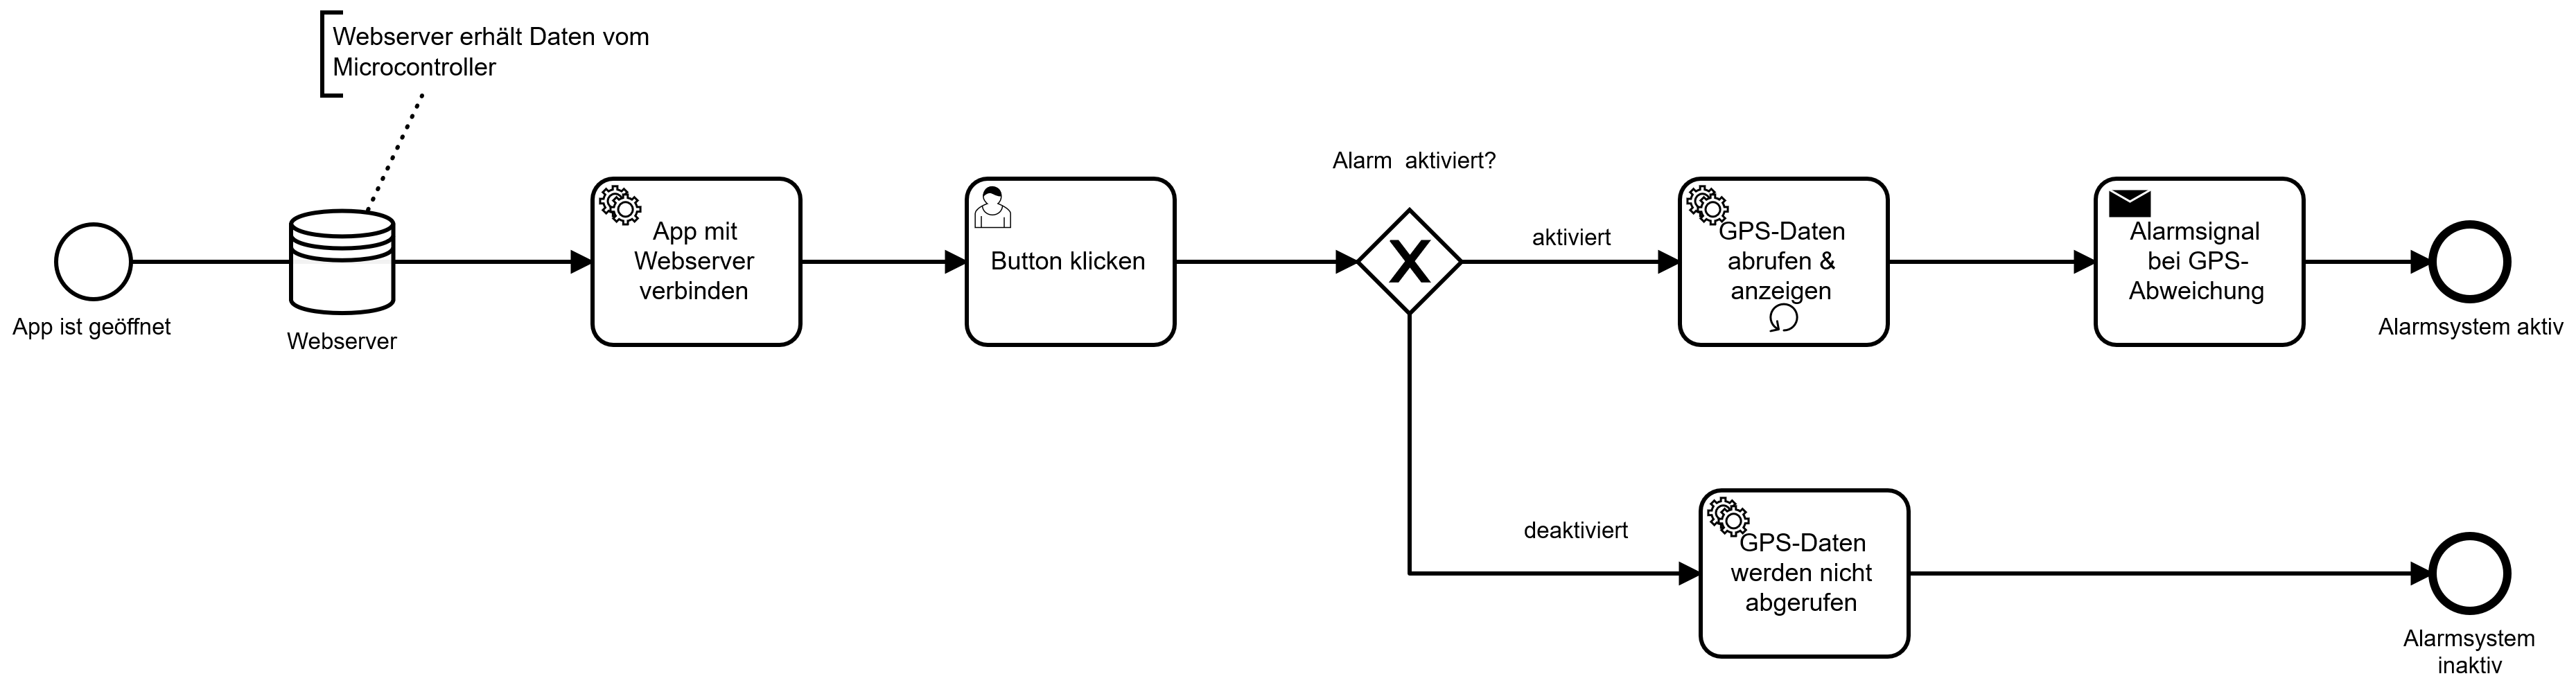
\includegraphics[width=1\textwidth]{Bilder/iOS_camunda.png}
		\caption{Entwurf der Hauptfunktionalitäten}
		\label{camunda}
	\end{center}
\end{figure}
\clearpage

\subsection{Design}
Das Design der beiden Apps unterscheidet sich stark und das wurde auch bewusst von uns zugelassen - es war uns wichtig, Hauptkriterien der Funktionalitäten zu definieren, wie beispielsweise in Abbildung \ref{camunda} zu sehen, aber der Kreativität jedes einzelnen von uns wollten wir keine Grenzen vorschreiben.
\\
\begin{center}
	\textit{Kreativ werden wir dann, wenn wir unsere immer gleichen Muster, unsere üblichen Gedankenabläufe unterbrechen und unseren Geist auf ungewohnte Wege schicken}\footcite{Bode2022}
\end{center}
Der Stil dieser App, besticht durch sein sehr minimalistisches und dennoch durch moderne Farben geprägtes Design. Wir haben hierbei auf Intuitivität geachtet und auf  \textit{viel Text} verzichtet, da die App so keine möglichen Sprachbarrieren aufwirft und zeitgemäßer wirkt.
\\
\\
Unscheinbar aber wichtig! Der Nutzer sieht als erstes das AppIcon im Appstore sowie später auf seinem Bildschirm. Hierbei wollten wir erreichen, dass dieses Icon nicht nur zu unserem Produkt passt, sondern auch optisch sehr anspricht. Daher haben wir uns für ein Icon entschieden, welches die Farben der iOS-App enthält sowie ein Auto, wie in Abbildung \ref{AppIcon}  demonstriert.
\begin{figure} [H]
	\begin{center}
		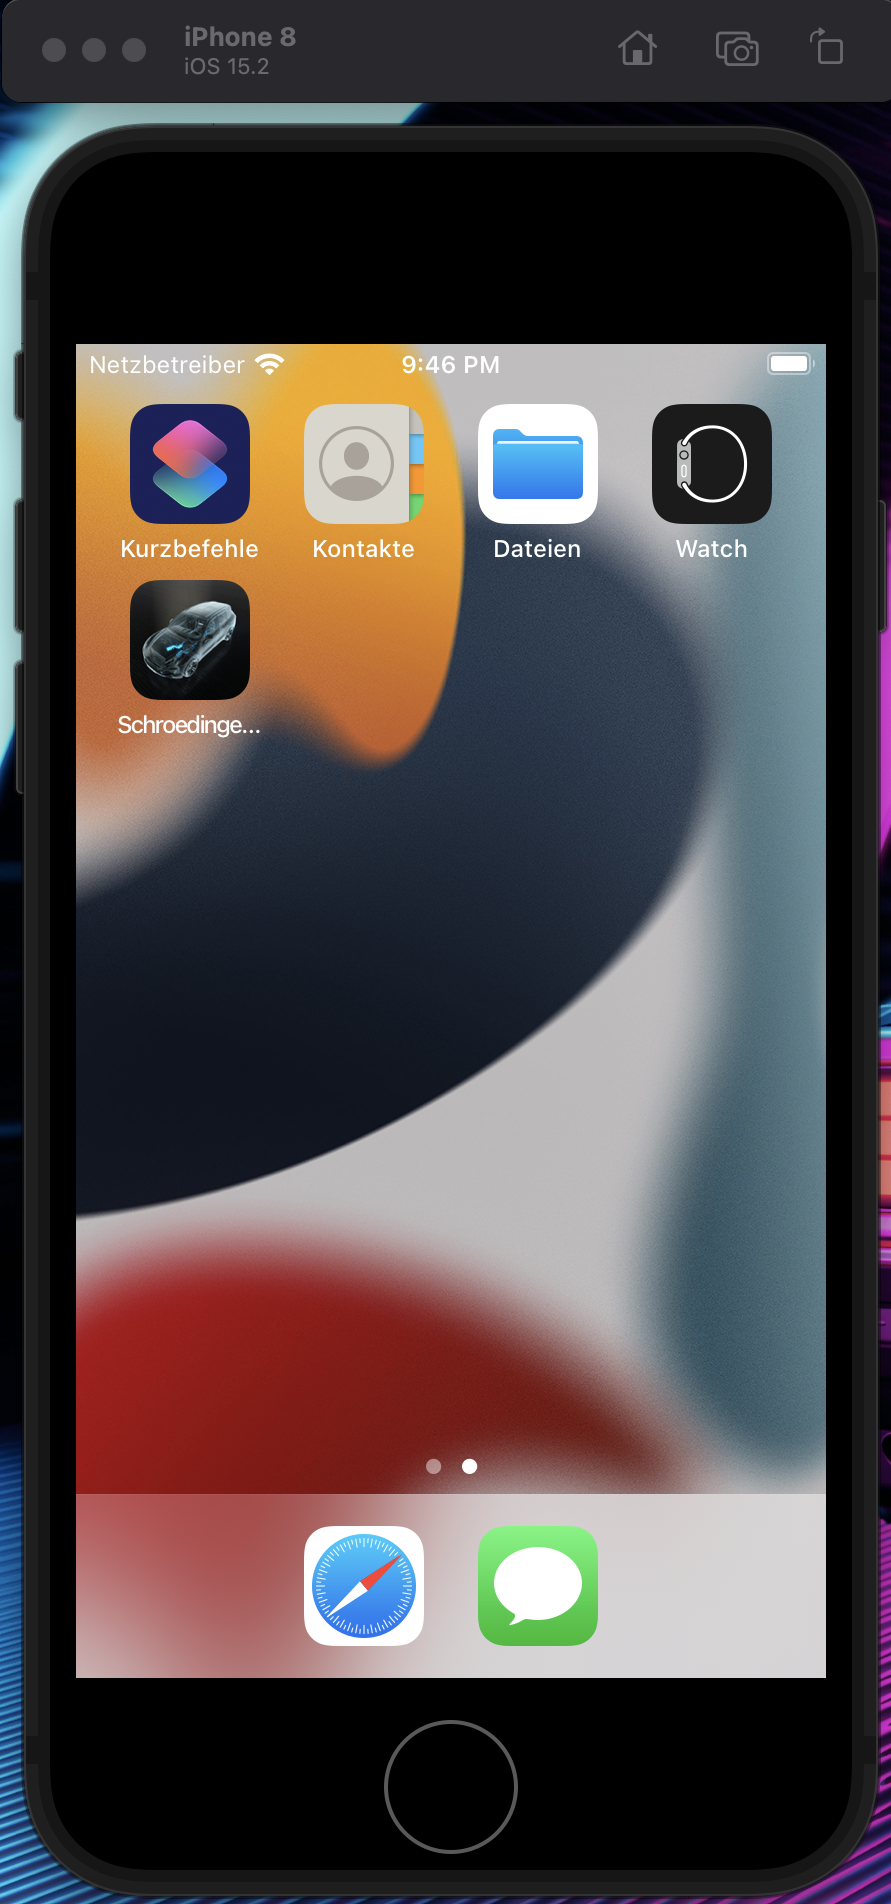
\includegraphics[width=0.4\textwidth]{Bilder/iOS_icon.png}
		\caption{AppIcon auf dem Bildschirm}
		\label{AppIcon}
	\end{center}
\end{figure}
Nach dem berühmten Tap auf das Icon hängt es oftmals vom Alter des genutzten Gerätes ab, wie schnell eine App sich aufbaut. Damit auch hier der User ein Feedback erhält, ob  etwas passiert, haben wir einen Launchscreen implementiert, welcher ebenfalls dem Design der App entspricht.(Abbildung \ref{Launch})
\begin{figure} [H]
	\begin{center}
		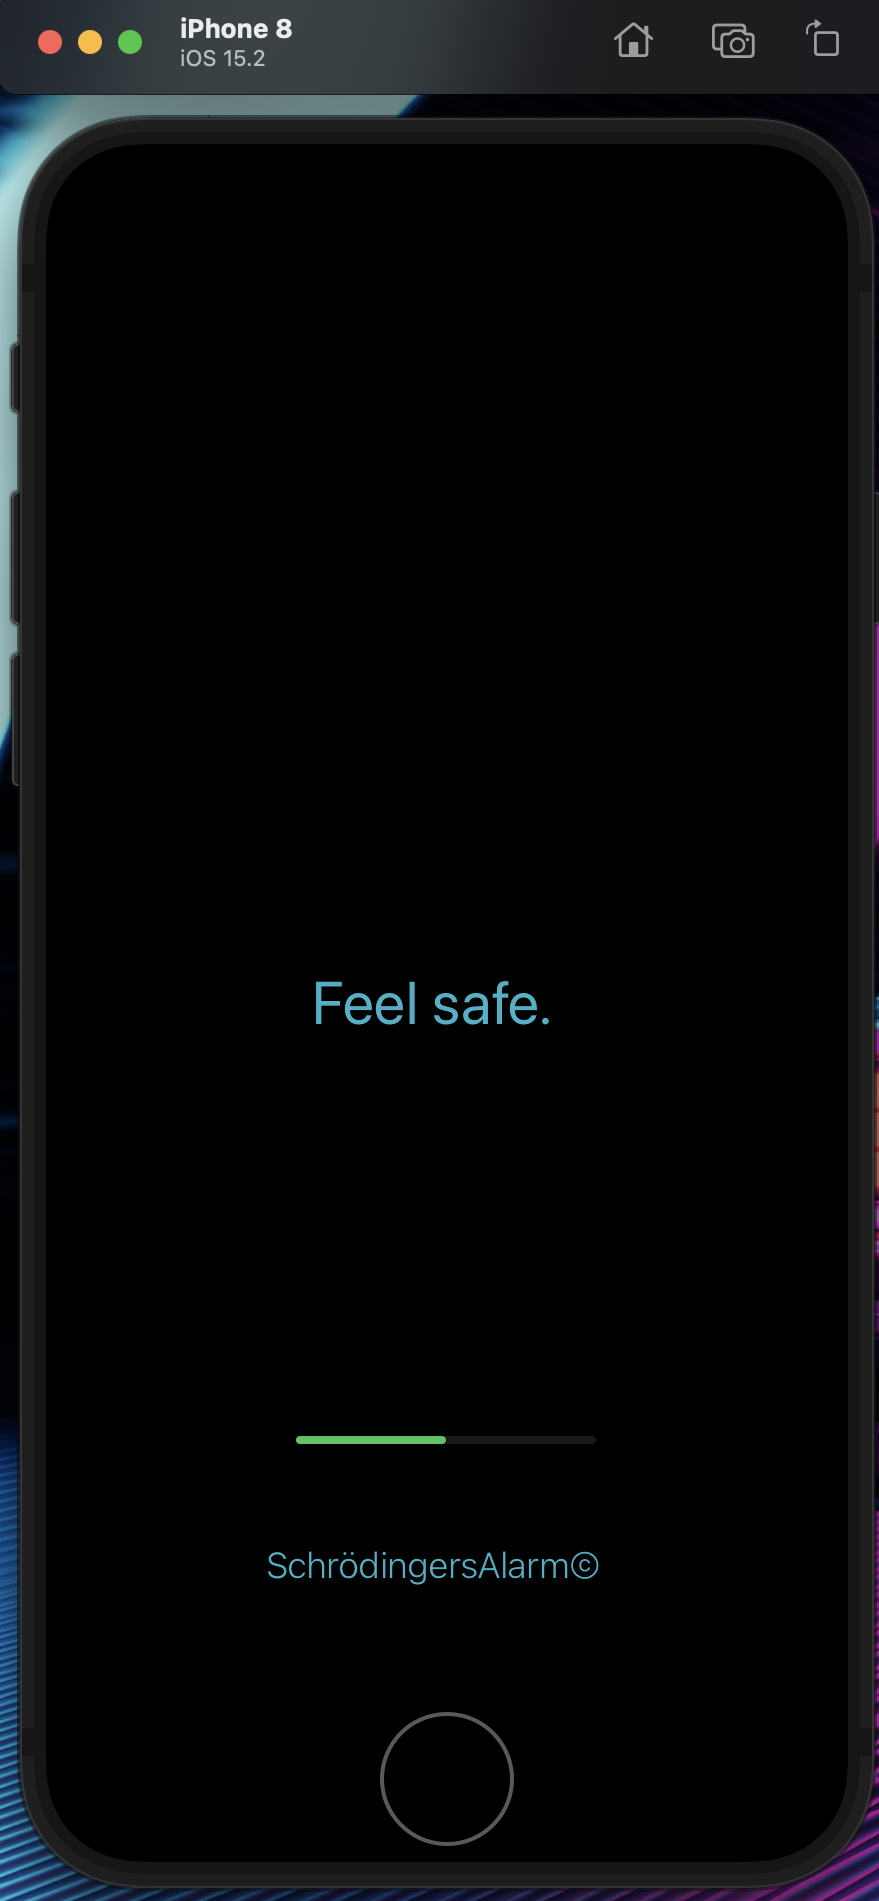
\includegraphics[width=0.4\textwidth]{Bilder/iOS_launch.png}
		\caption{Launchscreen}
		\label{Launch}
	\end{center}
\end{figure}
Beim Blick auf den Home-Bildschirm, im Navigations-Menü am kleinen Häuschen unten auf Daumenhöhe zu erkennen, sticht sofort das große Schloss ins Auge. Dieses kann auch wortwörtlich verstanden werden - ist es grün, dann ist der Alarm aktiviert \textit{(verschlossen, gesichert)}, tapt der Nutzer erneut darauf, ist es rot und der Alarm deaktiviert \textit{(geöffnet, ungesichert)}.
\begin{figure} [H]
	\begin{center}
		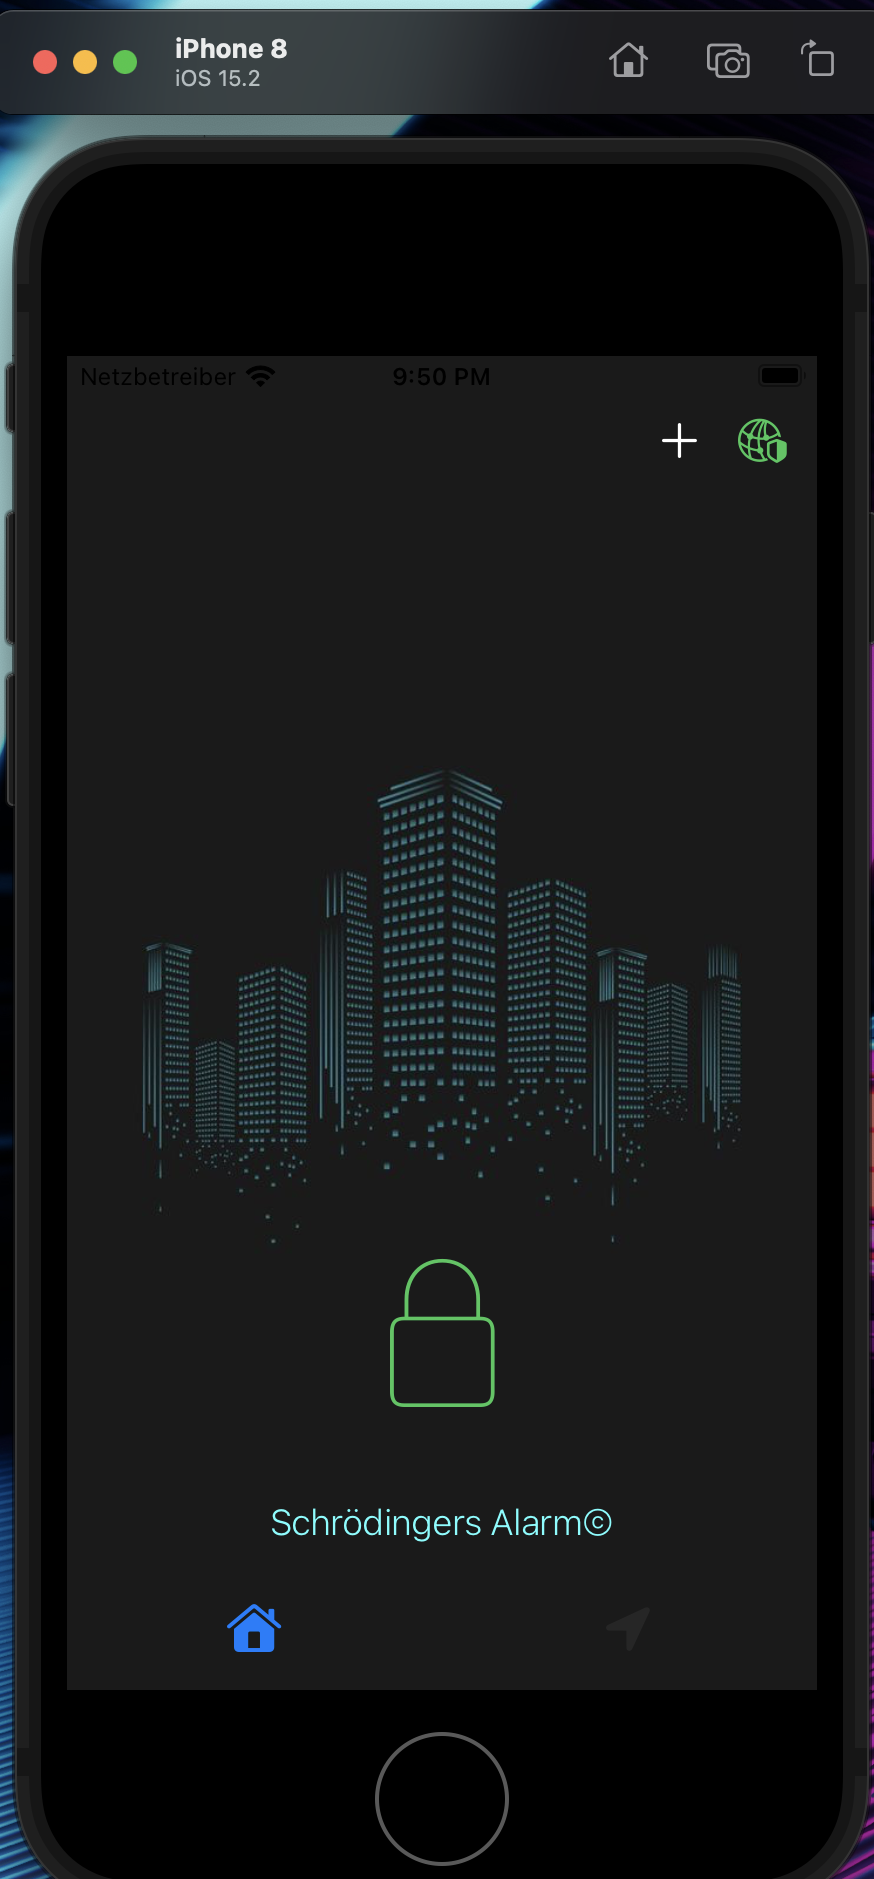
\includegraphics[width=0.4\textwidth]{Bilder/iOS_home.png}
		\caption{Navigationstab \textit{Home im aktivierten Modus}}
		\label{lock}
	\end{center}
\end{figure}
Bei der Umsetzung  des Kartendesigns war es wichtig, dass der Nutzer die vom Server bereitgestellten Daten angezeigt bekommt. Das  Feature, dass diese nicht als plain-Text dargestellt, sondern die Koordinaten direkt als Standort auf einer Karte übersetzt werden, haben wir ebenfalls umgesetzt, wie in Abbildung \ref{Map} visualisiert.
\begin{figure} [H]
	\begin{center}
		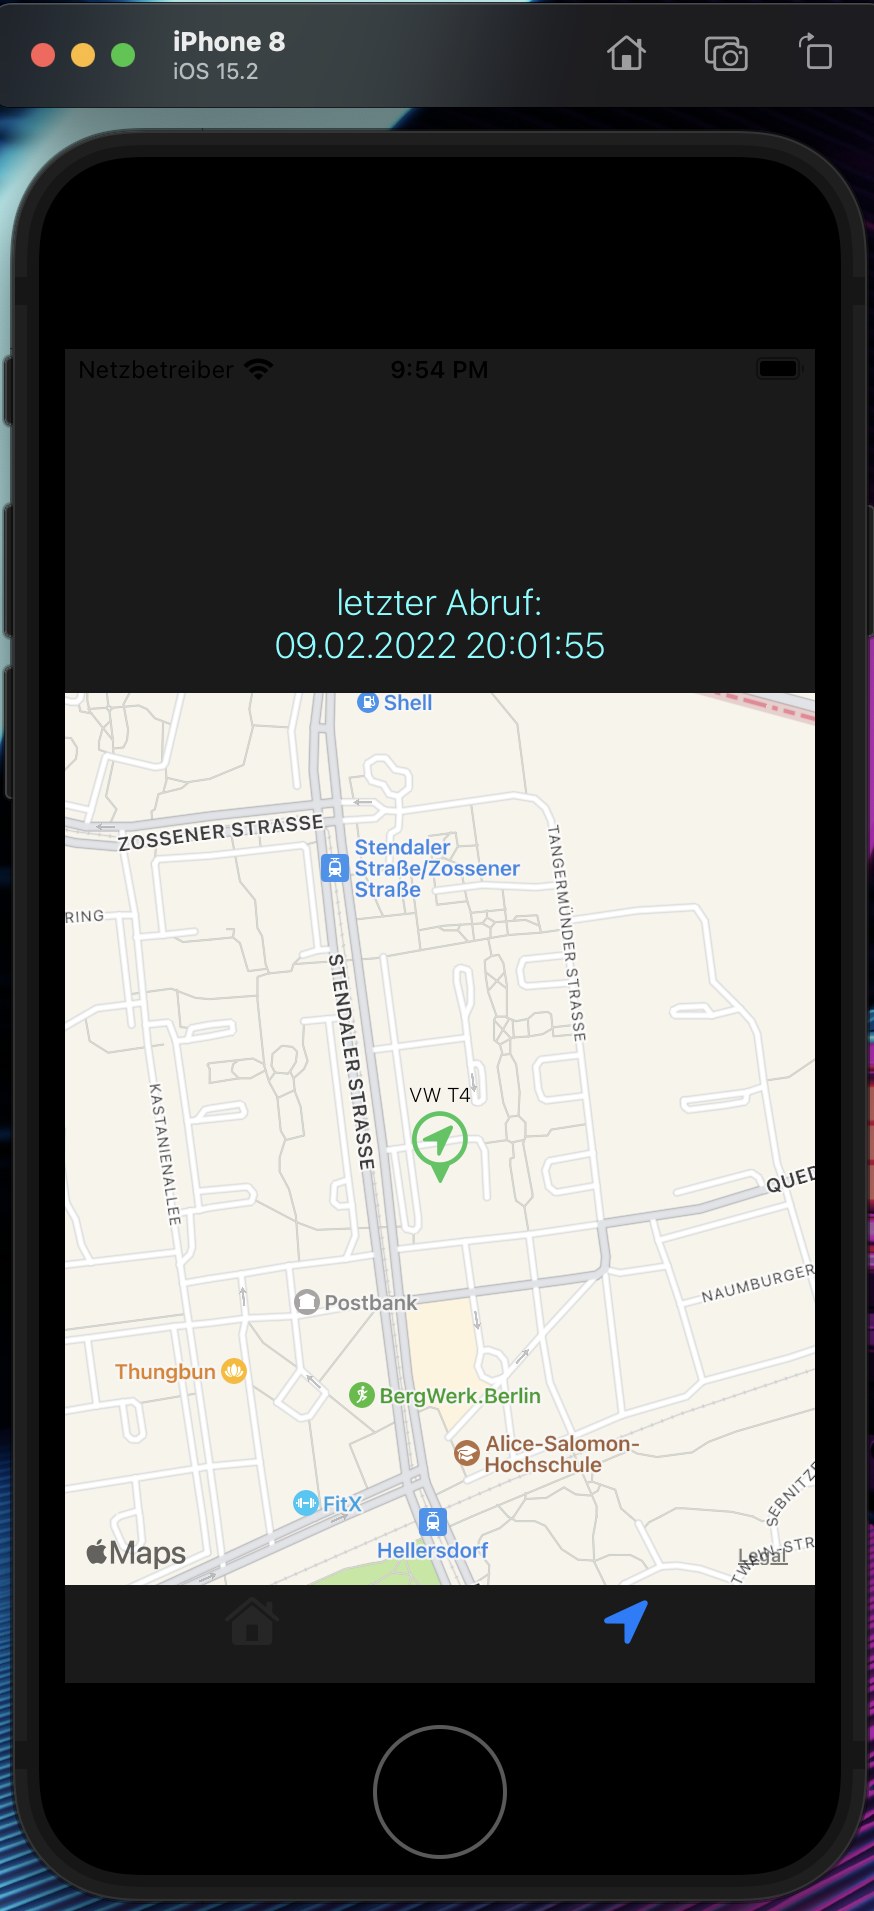
\includegraphics[width=0.4\textwidth]{Bilder/iOS_map.png}
		\caption{Navigationstab \textit{Map}}
		\label{Map}
	\end{center}
\end{figure}
Zur noch besseren Vorstellung, wie das Handling der beiden Apps ist, sind unter \textbf{Anhänge} die Links zu den jeweiligen auf Youtube hochgeladenen Demonstrations-Videos hinterlegt.



\subsection{Probleme}
Wie bereits angedeutet, gab es bei der Entwicklung einige Probleme, es waren kleinere wie anfänglich kein ausreichend leistungsstarkes und zudem mit aktuellem Betriebssystem ausgestattetem Macbook und größere, wie nachfolgend genauer beschrieben.
\\
\\
\subsubsection{Koordinaten in JSON als String hinterlegt}

Zu Beginn wurden die Koordinaten, sowie der Abrufzeitpunkt als Strings vom Server zur Verfügung gestellt, was ein Parsen sehr erschwerte, da für die Verarbeitung dieser Daten die iOS-Map integer beziehungsweise double-Werte benötigt. Dieses Problem konnte jedoch nach interner Rücksprache schnell behoben werden, da es sich lediglich um eine Einstellung beim Encode des Webservers handelte.

\subsubsection{Http? Abrufen verboten!}

Die benötigten Daten vom Server werden nicht innerhalb der App angezeigt und es erweckte auch nie den Anschein, dass diese überhaupt abgerufen werden. Es wurde sehr lange das Problem innerhalb der Methoden gesucht, jedoch ohne nennenswerte Erkenntnisse. Erst als extern um Hilfe gebeten wurde, kam schnell heraus, dass SwiftUI den Abruf von JSON-Daten einer Http-Seite verhindert. Nach gezielter Platzierung von print()-Ausgaben im Log wurde das eigentliche Problem sichtbar, siehe Abbildung \ref{fehler}. Bei Nutzung einer Beispiel JSON-Datei von einer Https-Seite trat keine Fehlermeldung mehr auf.
\begin{figure} [H]
	\begin{center}
		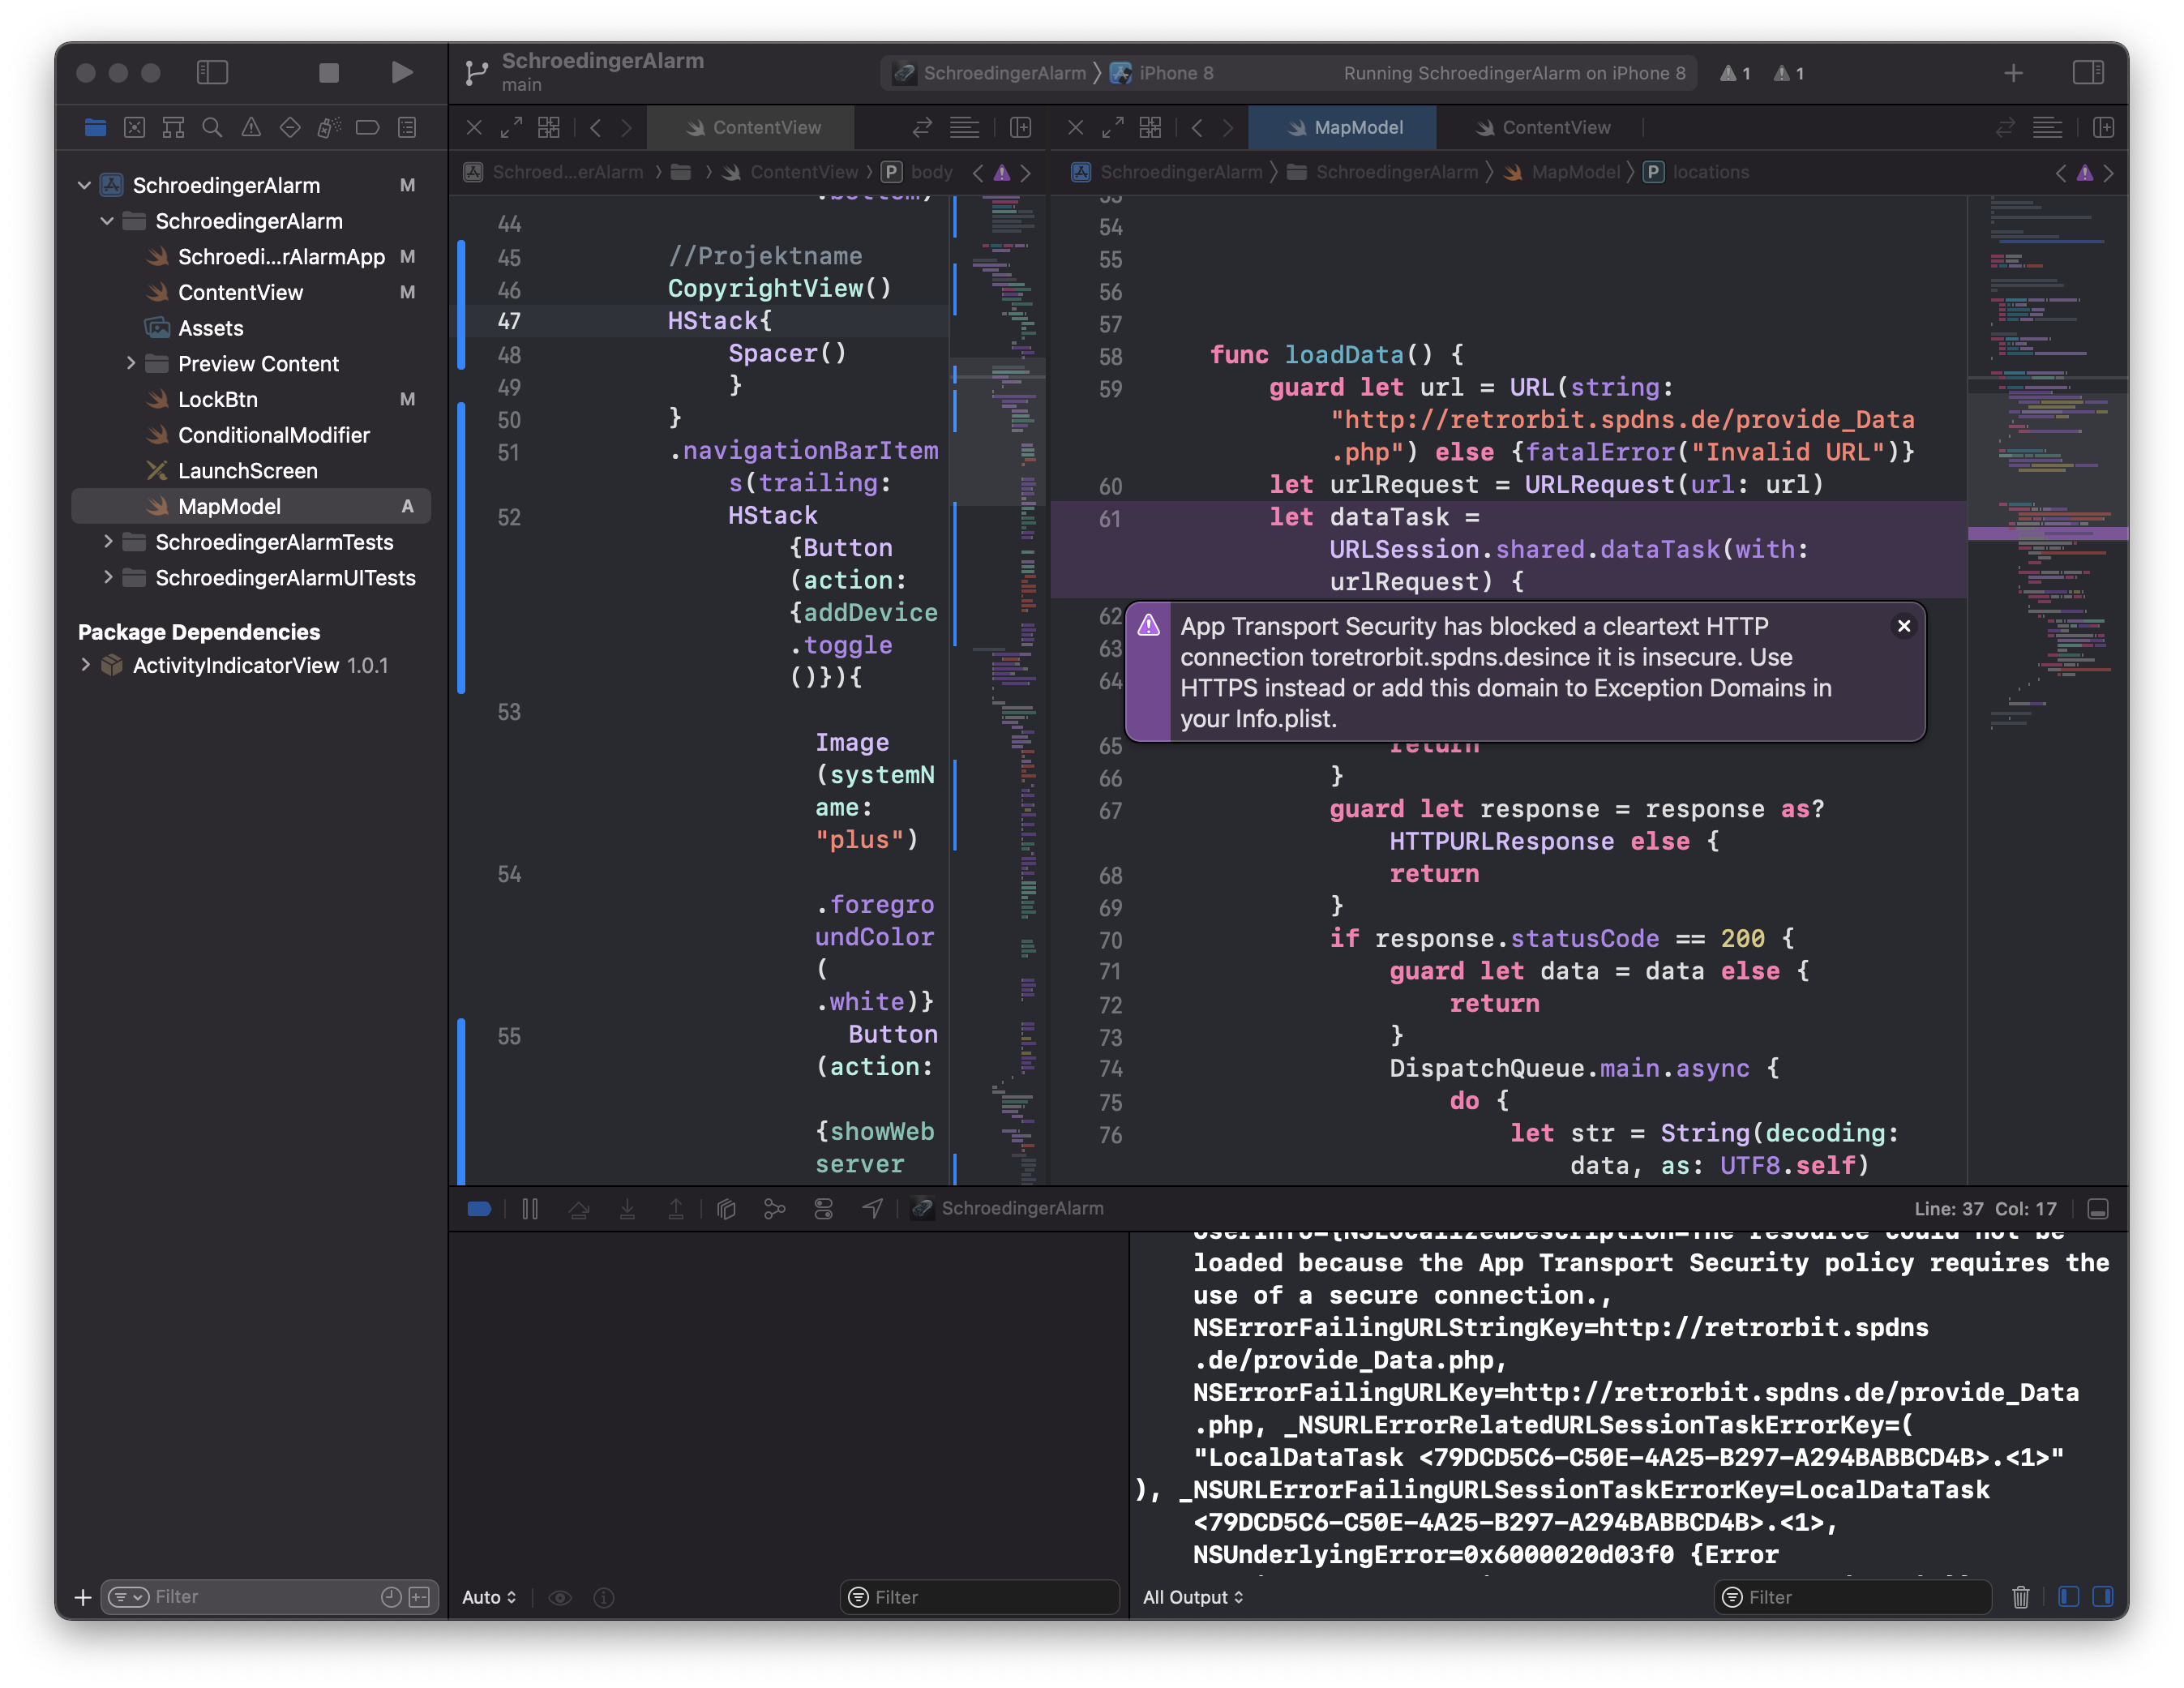
\includegraphics[width=1\textwidth]{Bilder/iOS_fehlermeldung.png}
		\caption{Fehlermeldung \textit{NSAppTransportSecurity}}
		\label{fehler}
	\end{center}
\end{figure}
Auf Apple-Plattformen verbessert eine Netzwerkfunktion namens App Transport Security (\textit{ATS}) den Datenschutz und die Datenintegrität für alle Apps und App-Erweiterungen. ATS erfordert, dass alle HTTP-Verbindungen, die mit dem URL-Ladesystem hergestellt werden – normalerweise unter Verwendung der URLSession-Klasse – HTTPS verwenden. Es erlegt außerdem erweiterte Sicherheitsprüfungen auf, die die vom TLS-Protokoll\footnote{Transport Layer Security} vorgeschriebene Standard-Server-Vertrauensbewertung ergänzen. ATS blockiert Verbindungen, die die Mindestsicherheitsanforderungen nicht erfüllen. [..] Diese Schutzmaßnahmen können umgangen werden, indem der NSAppTransportSecurity-Schlüssel zur Information Property List-Datei der App hinzugefügt und ein ATS-Konfigurationswörterbuch als Wert angegeben wird \cite{Inc}
\\
\\
Dieses Problem kann also behoben werden, wurde aber leider nicht mehr innerhalb der Bearbeitungszeit geschafft und wird später nachgeholt.	
	\chapter{Produkt}
	Unser Prototyp setzt sich derzeit aus 3 Systemen zusammen: dem Arduino samt Shield für die Möglichkeit der Ortung und Simkartenslot, den Webserver zur Datenverteilung und -bereitstellung sowie eine App für die Smartphone Betriebssysteme Android und iOS.

\textbf{Bild (Raspi, Arduino, Smartphones mit geöffneter App)}

\section{zukünftiges Produktangebot}
Wir haben uns zwei Produktkategorien überlegt, mit denen wir Gewinn generieren können. Zum einen ist das ein monatliches Bezahlkonzept. Hierbei haben wir uns an dem Konzept einiger Mobilfunkanbieter orientiert. Die Überlegung ist, dass wir zwei hinzu buchbare Optionen anbieten und man nur das bezahlt, was wirklich gebraucht wird. Eine Optionen ist die Google Standort API für eine genauere und zuverlässigere Standorterkennung. Die andere Option ist das Bestellen einer Sim-Karte mit Mobilfunkvertrag. Die Idee ist hier, dass so gegen einen kleinen Aufpreis der Ease-of-Use unseres Produkts weiter gesteigert wird.

Für das Endgerät haben wir uns neben der aktuellen Basis Variante für eine Base+ und eine Pro Variante entschieden. Bei der Base+ Variante ergänzen wir die Basis Variante lediglich um eine Sirene und etwas mehr Akkuleistung. Für die Pro Variante erweitern wir das Basismodell um einen WLAN Empfänger. Des Weiteren überlegen wir unseren modularen Aufbau für eine weitere Umsatzsteigerung zu nutzen und Akkumodule zu verkaufen, mit denen die Akkulaufzeit unserer Produkte vom Nutzer beliebig verlängert werden kann. Ein weiterer Vorteil ist, dass so bei nachlassender Akkuleistung unser Produkt nicht entsorgt werden muss, sondern der Nutzer einfach mit offiziellen Produkten den Akku wechseln kann. Dies soll verhindern, dass der Kunde auf Drittanbieter zurückgreift.
Das Ziel ist, dass wir unsere Apps und den Webserver unabhängig von der Produktversion verwenden können.

\section{Vergleich} 
Eine kurze Suche im Internet nach ähnlich funktionierenden  Systemen lässt schnell die Frage aufkommen : 
Wo liegt bei uns der Unterschied?
Für die direkte Konkurrenzanalyse haben wir uns für den Platzhirsch Amazon entschieden, da es wahrscheinlich nirgendwo sonst so viele ähnliche Produkte aus den unterschiedlichsten Ländern mit diversen Qualitätsmerkmalen gibt. Wir haben dafür Produkte im niedrigeren  Preissegment für rund 30€, im mittleren für rund 60€ und im höherpreisigen für weit über 100€ mit unserem verglichen. 

\begin{figure} [H]
	\begin{center}
		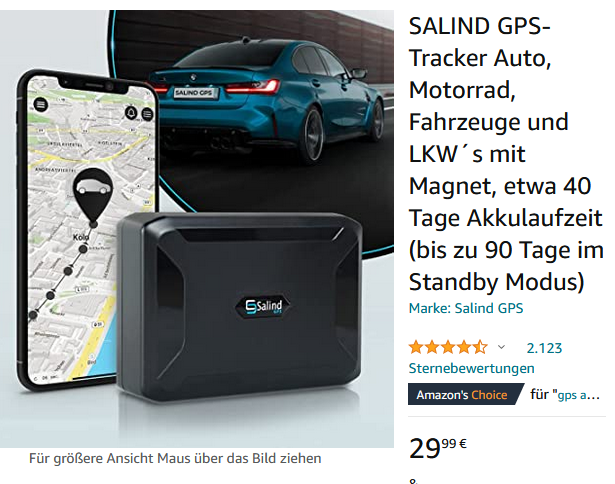
\includegraphics[width=0.75\textwidth]{Bilder/Produkt_Vergleich.png}
		\caption{Vergleichsprodukt im unteren Preissegment}
		\cite{Salind}
		\label{product_vgl}
	\end{center}
\end{figure}

Es lässt sich festhalten, dass alle Systeme die gleiche Grundfunktion besitzen: eine App, mit der das sich im Auto befindliche Gerät über einen Server Koordinaten-Daten abrufen und auswerten kann. Dennoch sind uns wesentliche Punkte aufgefallen, die sich abheben:

\begin{itemize}
	\item unser System ist nicht fest in sich verbaut, das bedeutet bei möglichen Defekten kann es leicht geöffnet werden und bei Bedarf einfach selbstständig repariert werden
	\item Die Akkus sind austauschbar und können mit einem handelsüblichen Ladegerät bequem daheim aufgeladen werden, so muss das Gesamtsystem nicht aus dem Auto entnommen werden. Anmerkung: alle Systeme, die wir uns angesehen haben, haben festverbaute Akku Systeme, die nur über Micro USB aufgeladen werden können
	\item Aus diesen Punkten ergibt sich auch direkt der nächste positive Effekt: da alle Bestandteile leicht zugänglich und austauschbar sind, ist unser Produkt sehr viel nachhaltiger - zudem haben wir auf unnötige Kunststoff Bestandteile verzichtet
	\item Des weiteren ist unser System durch sein offenherziges Design leicht erweiterbar und erinnert so unter anderem an die Uridee des \textit{Fairphone} mit seiner Komponenten Bauweise: man kauft nur, was man braucht, erhält aber garantiert ein funktionierendes Basissystem.
	\item Ebenfalls geht man bei unserem Produkt keine aufgezwungene Vertragspartner Bindung ein - der Internetanbieter kann sich der Kunde selbst aussuchen
\end{itemize}
Es lässt sich daher behaupten - Ja, Produkte wie dieses sind in der Basis nicht neu, dennoch haben wir uns Gedanken in ganz unterschiedliche Richtungen gemacht und unseren Ideenhorizont frei gehalten, so dass sich unser Produkt stetig mit und für den Kunden weiterentwickeln kann.

	\chapter{Rück- und Ausblick}
	\input{Rück_Ausblick}
	
	\addcontentsline{toc}{chapter}{Abbildungsverzeichnis}	
	\listoffigures
	%\addcontentsline{toc}{chapter}{Tabellenverzeichnis}	
	%\listoftables
	%\printbibliography[heading=bibintoc]
	\printbibliography[heading=bibintoc, title={Quellenverzeichnis}]
\end{document}